% =====================================================================
% TmFeO3 Fe-Tm K^- Coupling: physical-J -> PJP -> local SU(3) lambda basis
% Restored gauge-covariant derivation with implementation guidance
% =====================================================================
\documentclass[11pt,a4paper]{article}

\usepackage{amsmath,amssymb,mathtools,bm}
\usepackage{graphicx}
\usepackage{geometry}
\geometry{margin=2.2cm}
\usepackage{booktabs,array,longtable}
\usepackage{xcolor}
\usepackage{hyperref}
\hypersetup{colorlinks=true,linkcolor=blue,citecolor=blue,urlcolor=blue}
\usepackage{cleveref}
\usepackage{tikz}
\usetikzlibrary{arrows.meta,positioning,calc,decorations.pathmorphing}
\usepackage{tcolorbox}
\tcbuselibrary{skins,breakable}

\newtcolorbox{keybox}[1][]{colback=orange!8!white,colframe=orange!70!black,fonttitle=\bfseries,title={Key point},breakable,#1}
\newtcolorbox{warnbox}[1][]{colback=red!6!white,colframe=red!70!black,fonttitle=\bfseries,title={Warning},breakable,#1}
\newtcolorbox{implbox}[1][]{colback=blue!5!white,colframe=blue!60!black,fonttitle=\bfseries,title={Implementation prescription},breakable,#1}

\newcommand{\Fe}{\mathrm{Fe}}
\newcommand{\Tm}{\mathrm{Tm}}
\newcommand{\diag}{\mathrm{diag}}
\newcommand{\ket}[1]{|#1\rangle}
\newcommand{\bra}[1]{\langle #1|}
\newcommand{\braket}[2]{\langle #1|#2\rangle}
\newcommand{\ve}[1]{\boldsymbol{#1}}
\newcommand{\lam}[1]{\lambda^{#1}}
\newcommand{\lvecminus}{\boldsymbol{\lambda}^{-}}
\newcommand{\lvecplus}{\boldsymbol{\lambda}^{+}}
\newcommand{\Rz}{R_z(\pi)}
\newcommand{\Rx}{R_x(\pi)}
\newcommand{\Ry}{R_y(\pi)}

\title{\textbf{TmFeO$_3$ Fe--Tm $K^-$ Coupling}\
\large Restored derivation: physical $J$ operator, $PJP$ projection, local SU(3) qutrit basis, transported-gauge bond formulas, and the physical cross-peak mechanism (vertices, conservation laws, Liouville pathways), grounded in measured TmFeO$_3$ parameters}
\author{Working note}
\date{June 2026}

\begin{document}
\maketitle
\tableofcontents
\bigskip

% =====================================================================
\section{Purpose and conceptual reset}
% =====================================================================

The goal of this note is to formulate the Fe--Tm coupling in a way that is
mathematically well-defined all the way down to the projected qutrit operators.
The central object is the $K^-$ coupling, namely the bilinear coupling between
an Fe spin and the time-reversal-odd Tm qutrit operators
\begin{equation}
  \lvecminus_j =
  \begin{pmatrix}
    \lambda_j^2\\ \lambda_j^5\\ \lambda_j^7
  \end{pmatrix}.
\end{equation}
The superscript ``$-$'' means time-reversal odd.  The notation $j$ labels the
Tm sublattice, not a spatial vector component.

\begin{keybox}
There are three different mathematical objects that must not be confused:
\begin{enumerate}
  \item $\ve S_i$: an Fe spin vector, stored in global crystallographic axes.
  \item $\ve J_j$: the physical Tm angular momentum operator in the full $J=6$ Hilbert space.
  \item $\lambda_j^a$: a coordinate operator in the local three-level qutrit basis at Tm sublattice $j$.
\end{enumerate}
Only $\ve S$ and the full $\ve J$ are axial vectors.  A Gell-Mann operator $\lambda_j^a$ is not a spatial vector component.  It transforms by the adjoint action induced by the chosen qutrit bases.
\end{keybox}

The physically supported route is therefore
\begin{equation}
  \boxed{
  \text{physical }\ve S\text{ and }\ve J
  \quad\longrightarrow\quad
  H_{\Fe-\Tm}=\ve S^T A\ve J
  \quad\longrightarrow\quad
  P_j\ve J P_j
  \quad\longrightarrow\quad
  K^-_{ij}\lvecminus_j .}
\end{equation}
One should not start by assuming that the space-group rotation $R_x(\pi)$ acts as a closed onsite SU(3) rotation in one fixed Tm qutrit.  That is precisely the dangerous shortcut.

% =====================================================================
\section{Physical system: verified TmFeO$_3$ parameters}
\label{sec:tmfeo3-facts}
% =====================================================================

Before any formal manipulation we fix the physical setting and the numbers the
model is calibrated against.  All values below are experimental properties of
bulk TmFeO$_3$; the simulation parameters sit close to them, and the small
residual differences are stated explicitly so that ``model'' and
``measurement'' are never silently conflated.

\paragraph{Structure and sites.}
TmFeO$_3$ is an orthorhombically distorted perovskite, space group $Pbnm$
(No.\ 62, a nonstandard setting of $Pnma$), with $Z=4$ formula units per cell.
The Fe$^{3+}$ ions occupy the Wyckoff $4b$ sites, whose site symmetry is
$\bar 1$: \emph{each Fe sits on an inversion centre}, so spatial inversion maps
every Fe sublattice to itself.  The Tm$^{3+}$ ions occupy the $4c$ sites
$(x,y,\tfrac14)$, whose site symmetry is the single mirror $m$ (the plane
$z=\tfrac14$, i.e.\ $m_z$); inversion therefore exchanges Tm sublattices in
pairs.  This is exactly the Fe/Tm permutation structure used in the
Pbnm-ingredients section, and it is dictated by the crystallography, not
chosen.  In particular, the local mirror $m_z=S_1^{-1}I$ that generates the
$\lambda^5,\lambda^7$ sign is the physical $4c$ site mirror.

\paragraph{Magnetic ions.}
Fe$^{3+}$ is $3d^5$, a spin-only $^6S_{5/2}$ ion ($S=5/2$, $L\approx0$,
$g\approx2$), represented classically by the unit vector $\ve S_i$.
Tm$^{3+}$ is $4f^{12}$ with ground multiplet $^3H_6$ ($J=6$, $13$ states).  In
the $C_s(m)$ crystal field the multiplet splits into $13$ \emph{singlets}
(a non-Kramers ion in a site without rotational degeneracy has no protected
doublets); the qutrit keeps the three lowest, $\ket{E_1},\ket{E_2},\ket{E_3}$,
and represents them by local SU(3) Gell-Mann operators.

\paragraph{Magnetic order and the $\Gamma_2$ ground state.}
The Fe sublattice orders G-type antiferromagnetically at
$T_N\approx 632\,\mathrm K$, with a Dzyaloshinskii--Moriya canting that
produces weak ferromagnetism.  In Bertaut/Yamaguchi mode
notation~\cite{Yamaguchi} the relevant collinear-mode multiplets are
\begin{equation}
  \Gamma_2=(F_x,C_y,G_z),\qquad
  \Gamma_4=(G_x,A_y,F_z).
\end{equation}
On cooling, TmFeO$_3$ undergoes a continuous spin reorientation
$\Gamma_4\!\to\!\Gamma_{24}\!\to\!\Gamma_2$ between $T_2\approx85\,\mathrm K$
and $T_1\approx93\,\mathrm K$~\cite{Zhang2016,Kimel2004}.  Below
$\sim85\,\mathrm K$ the equilibrium is $\Gamma_2$: the main AFM vector $\ve G$
lies along $c$ ($G_z$) and the weak ferromagnetic moment $\ve F$ along $a$
($F_x$).  This $F_x+G_z$ state is the ``baseline'' used throughout the
numerical sections.

\paragraph{Excitation energies: the two axes of the cross peak.}
The two THz excitations that define the target cross peak are an Fe magnon and
a Tm crystal-field transition:
\begin{center}
\renewcommand{\arraystretch}{1.25}
\begin{tabular}{lcccl}
\toprule
Excitation & THz & meV & cm$^{-1}$ & role \\
\midrule
Fe quasi-FM magnon        & $0.28$        & $1.16$        & $9.3$        & low Fe mode \\
Fe quasi-AFM magnon       & $0.86$        & $3.56$        & $28.7$       & pumped $q_{\mathrm{AFM}}$ ($\omega_\tau$ axis) \\
Tm CEF $E_{12}$ ($R_1$)   & $0.52$        & $2.15$        & $17.3$       & detected coherence ($\omega_t$ axis) \\
Tm CEF $E_{23}$ ($R_2$)   & $0.61$        & $2.52$        & $20.3$       & sets $\Delta_{13}$ with $E_{12}$ \\
Tm CEF $E_{13}$ ($R_3$)   & $1.15$        & $4.76$        & $38.4$       & third qutrit level \\
\bottomrule
\end{tabular}
\end{center}
Conversion factor: $1\,\mathrm{THz}=4.136\,\mathrm{meV}=33.36\,\mathrm{cm^{-1}}
=47.99\,\mathrm K$.  The three CEF lines are mutually consistent with a
three-singlet qutrit, $E_{12}+E_{23}\approx E_{13}$
($0.52+0.61\approx1.13\,$THz), so the onsite splittings in $H_{\Tm,0}$ are
$\Delta_{12}\approx0.52$ and $\Delta_{13}\approx1.13\,$THz.  The simulation
uses $q_{\mathrm{AFM}}\approx0.90$ and $E_{12}\approx0.50\,$THz, within a few
percent of the measured $0.86$ and $0.52\,$THz~\cite{Zhang2016,MP2018}.  The
cross-peak question is whether a coherence on the
$\omega_\tau=q_{\mathrm{AFM}}$ axis can be converted into a coherence on the
$\omega_t=E_{12}$ axis; the two differ by $\Delta\approx0.34\,$THz, a number we
return to under energy conservation in \cref{sec:mechanism}.

% =====================================================================
\section{Pbnm ingredients}
% =====================================================================

We use the generators
\begin{align}
  S_1 &: (x,y,z)\mapsto(-x,-y,z+\tfrac12),\\
  S_2 &: (x,y,z)\mapsto(x+\tfrac12,-y+\tfrac12,-z),\\
  I &: (x,y,z)\mapsto(-x,-y,-z).
\end{align}
For axial vectors, the corresponding spin-space matrices are
\begin{equation}
  R_{S_1}=\diag(-1,-1,+1)\equiv R_z,
  \qquad
  R_{S_2}=\diag(+1,-1,-1)\equiv R_x,
  \qquad
  R_I=\mathbf 1.
\end{equation}
Their product gives
\begin{equation}
  R_{S_1S_2}=R_y=\diag(-1,+1,-1).
\end{equation}
The sublattice permutations are
\begin{center}
\renewcommand{\arraystretch}{1.15}
\begin{tabular}{ccc}
\toprule
Operation & Fe sublattice action & Tm sublattice action\\
\midrule
$S_1$ & $(03)(12)$ & $(03)(12)$\\
$S_2$ & $(01)(23)$ & $(01)(23)$\\
$S_1S_2$ & $(02)(13)$ & $(02)(13)$\\
$I$ & identity & $(03)(12)$\\
\bottomrule
\end{tabular}
\end{center}
Thus inversion fixes each Fe sublattice but pairs Tm$_0\leftrightarrow$Tm$_3$ and Tm$_1\leftrightarrow$Tm$_2$.

% =====================================================================
\section{Full physical Fe--Tm exchange before projection}
% =====================================================================

Let a Fe--Tm bond be denoted
\begin{equation}
  b=(i,j;\ve n),
\end{equation}
where $i$ is an Fe sublattice, $j$ is a Tm sublattice, and $\ve n$ is the Tm-cell offset relative to the Fe cell.
Before any qutrit truncation, the most general bilinear physical exchange is
\begin{equation}
  \boxed{
  H_b^{\rm phys}=\ve S_i^T A_b\ve J_j .}
  \label{eq:phys-exchange}
\end{equation}
Here $A_b$ is a real $3\times3$ tensor with rows labelled by Fe spin components and columns labelled by Tm angular-momentum components:
\begin{equation}
  A_b=
  \begin{pmatrix}
    A_{xx}&A_{xy}&A_{xz}\\
    A_{yx}&A_{yy}&A_{yz}\\
    A_{zx}&A_{zy}&A_{zz}
  \end{pmatrix}_b.
\end{equation}

Under a space-group operation $g$, the physical axial vectors transform as
\begin{equation}
  \ve S_i\mapsto R_g\ve S_{\sigma_g^\Fe(i)},
  \qquad
  \ve J_j\mapsto R_g\ve J_{\sigma_g^\Tm(j)}.
\end{equation}
Therefore invariance of \cref{eq:phys-exchange} requires
\begin{equation}
  \boxed{A_{gb}=R_g^T A_b R_g.}
  \label{eq:A-covariance}
\end{equation}
This equation is safe because it is written in the full physical Hilbert space.  No SU(3) truncation has been used.

\begin{warnbox}
The statement that $\ve J$ is an axial vector is a statement about the full $J=6$ angular-momentum operator.  It is not a statement that $(\lambda^2,\lambda^5,\lambda^7)$ form a spatial vector.
\end{warnbox}

% =====================================================================
\section{Local qutrit bases and the $PJP$ projection}
% =====================================================================

At each Tm sublattice $j$, define the local qutrit projector
\begin{equation}
  P_j=\sum_{n=1}^{3}\ket{E_{n,j}}\bra{E_{n,j}}.
\end{equation}
The local qutrit basis is
\begin{equation}
  \mathcal B_j=\{\ket{E_{1,j}},\ket{E_{2,j}},\ket{E_{3,j}}\}.
\end{equation}
The Gell-Mann operator at that Tm site is defined by
\begin{equation}
  \lambda_j^a
  =\sum_{m,n=1}^{3}\ket{E_{m,j}}(\lambda^a)_{mn}\bra{E_{n,j}}.
  \label{eq:local-lambda-def}
\end{equation}
Thus $\lambda_j^a$ is a local operator coordinate in the Tm qutrit.  It is not a component of a spatial vector.

The physical projected angular momentum is
\begin{equation}
  \widetilde J_{j,\alpha}=P_jJ_\alpha P_j.
\end{equation}
In the local qutrit basis it is expanded as
\begin{equation}
  \boxed{
  P_jJ_\alpha P_j
  =\sum_{a\in\{2,5,7\}}\mu_{j,\alpha a}\lambda_j^a .}
  \label{eq:PJP-local}
\end{equation}

\begin{keybox}[title={Lemma: why only $\lambda^2,\lambda^5,\lambda^7$ appear}]
The restriction of \eqref{eq:PJP-local} to the three \emph{antisymmetric}
Gell-Mann matrices is exact, not a small-multipole approximation, and it rests
on one physical fact specific to this system.  Tm$^{3+}$ is a non-Kramers
$4f^{12}$ ion at a site of symmetry $m$, so its CEF eigenstates are
nondegenerate singlets and can be chosen \emph{real} (time-reversal symmetric).
In any real basis the angular-momentum operator $J_\alpha$ is purely imaginary
and antisymmetric, hence $\bra{E_m}J_\alpha\ket{E_n}$ is imaginary and
antisymmetric.  The only imaginary-antisymmetric Gell-Mann matrices are
$\lambda^2,\lambda^5,\lambda^7$, so $P_jJ_\alpha P_j$ has \emph{no} component
on $\lambda^{1,3,4,6,8}$.  The time-odd ($\lambda^-$) versus time-even
($\lambda^+$) split used throughout this note is therefore a rigorous
consequence of time reversal acting on a real singlet basis, not a modelling
choice.
\end{keybox}

For a reference local basis, the projected moment matrix is
\begin{equation}
  \mu_0=
  \begin{pmatrix}
    0&2.3915&0.9128\\
    0&-2.7866&0.4655\\
    5.264&0&0
  \end{pmatrix},
  \qquad
  \text{columns }(2,5,7).
  \label{eq:mu0}
\end{equation}
Equivalently,
\begin{align}
  P_0J_xP_0 &=2.3915\lambda_0^5+0.9128\lambda_0^7,\\
  P_0J_yP_0 &=-2.7866\lambda_0^5+0.4655\lambda_0^7,\\
  P_0J_zP_0 &=5.264\lambda_0^2.
\end{align}

The physical magnetic moment is
\begin{equation}
  \ve m_j^{\Tm}=-g_J\mu_B P_j\ve J P_j.
\end{equation}
Thus a lab magnetic field couples to the projected moment as
\begin{equation}
  H_{B,\Tm}(t)
  =-g_J\mu_B\sum_{j,\alpha,a}B_\alpha(t)\mu_{j,\alpha a}\lambda_j^a.
\end{equation}
The coefficient $\mu_{j,\alpha a}$ carries all local-basis information.

% =====================================================================
\section{The actual SU(3) symmetry action: $W_g$ and $D_g$}
% =====================================================================

Let $g$ map Tm sublattice $j$ to $j'=\sigma_g^\Tm(j)$.  The exact qutrit-basis map is
\begin{equation}
  \boxed{
  [W_g^{(j)}]_{mn}=\bra{E_{m,j'}}U_g\ket{E_{n,j}}.}
  \label{eq:W-def}
\end{equation}
It acts on qutrit states as
\begin{equation}
  U_g\ket{E_{n,j}}=\sum_m\ket{E_{m,j'}}[W_g^{(j)}]_{mn}.
\end{equation}
It induces an adjoint action on qutrit operators:
\begin{equation}
  \boxed{
  U_g\lambda_j^aU_g^\dagger=\sum_b\left[D_g^{(j)}\right]_{ba}\lambda_{j'}^b,}
  \label{eq:D-def-operator}
\end{equation}
where
\begin{equation}
  \boxed{
  \left[D_g^{(j)}\right]_{ba}=\frac12\operatorname{Tr}\left[\lambda^b W_g^{(j)}\lambda^a W_g^{(j)\dagger}\right].}
  \label{eq:D-def}
\end{equation}

\begin{keybox}
$W_g^{(j)}$ acts on qutrit states.  $D_g^{(j)}$ acts on qutrit operators.  $R_g$ acts on physical spatial vector components.  These are different matrices in different spaces.
\end{keybox}

The projected moment covariance is
\begin{equation}
  U_g(P_jJ_\alpha P_j)U_g^\dagger
  =\sum_\beta R_{g,\alpha\beta}
  P_{j'}J_\beta P_{j'}.
\end{equation}
Substituting \cref{eq:PJP-local,eq:D-def-operator} gives
\begin{equation}
  \boxed{
  \sum_a \mu_{j,\alpha a}\left[D_g^{(j)}\right]_{ba}
  =\sum_\beta R_{g,\alpha\beta}\mu_{j',\beta b}.}
  \label{eq:mu-covariance-index}
\end{equation}
In matrix notation, if $D$ is defined by $\lambda^a\mapsto D_{ba}\lambda^b$, then
\begin{equation}
  \boxed{
  \mu_{j'}=R_g^T\mu_j\,D_g^{(j)T}.}
  \label{eq:mu-covariance}
\end{equation}
This is the more theoretically supported relation.  It replaces the unsafe shortcut $\lambda_{\rm global}=\mu^{-1}R\mu\lambda_{\rm local}$.

\begin{warnbox}
The matrix $\mu^{-1}R_x\mu$ is generally not the adjoint representation of a unitary qutrit rotation.  The operation $S_2$ maps one Tm sublattice to another; it need not act as a closed onsite operation in one fixed qutrit.  The remedy is to work with $W_g^{(j)}$ and $D_g^{(j)}$, or to choose transported bases that make selected $D_g^{(j)}$ trivial by construction.
\end{warnbox}

% =====================================================================
\section{Transported gauge: a practical but explicit convention}
% =====================================================================

Choose Tm$_0$ as the reference qutrit.  Define
\begin{align}
  \mathcal B_0&=\{\ket{E_{1,0}},\ket{E_{2,0}},\ket{E_{3,0}}\},\\
  \mathcal B_1&=U_{S_2}\mathcal B_0,\\
  \mathcal B_2&=U_{S_1S_2}\mathcal B_0,\\
  \mathcal B_3&=U_{S_1}\mathcal B_0.
\end{align}
This is the transported gauge.  In this gauge,
\begin{equation}
  D_{S_2}^{(0)}=D_{S_1S_2}^{(0)}=D_{S_1}^{(0)}=\mathbf 1 .
\end{equation}
After restricting to the corresponding transported maps, the proper-coset qutrit action is therefore absorbed into the basis definition.
This does not mean that $R_x$ acts trivially on the qutrit.  It means we chose the target qutrit basis to be the image of the source qutrit basis.

The physical global projected moment on site $j$ is then
\begin{equation}
  \boxed{
  P_jJ_\alpha^{\rm global}P_j
  =\sum_{\beta,a}(R_j)_{\alpha\beta}\mu_{0,\beta a}\lambda_j^a,}
  \label{eq:global-PJP-transported}
\end{equation}
where
\begin{equation}
  R_0=\diag(+,+,+),\quad
  R_1=\diag(+,-,-),\quad
  R_2=\diag(-,+,-),\quad
  R_3=\diag(-,-,+).
\end{equation}
This is how a global lab field talks to local Tm $\lambda_j$ operators in transported gauge:
\begin{equation}
  H_{B,\Tm}(t)=-g_J\mu_B\sum_{j,a}
  \left[\sum_{\alpha,\beta}B_\alpha(t)(R_j)_{\alpha\beta}\mu_{0,\beta a}\right]
  \lambda_j^a.
\end{equation}

% =====================================================================
\section{Local mirror and the origin of the $\lambda^5,\lambda^7$ sign}
% =====================================================================

Two operations map Tm$_0$ to Tm$_3$: $S_1$ and $I$.  In transported gauge the Tm$_3$ basis is defined with $S_1$.  Therefore the inversion map differs from the transported map by the local operation
\begin{equation}
  h=S_1^{-1}I.
\end{equation}
Using the coordinate maps,
\begin{equation}
  h:(x,y,z)\mapsto(x,y,-z+\tfrac12),
\end{equation}
which is a local mirror $m_z$ up to a translation.

For a $J_z$ basis state, the mirror can be written as $m_z=IC_{2z}$.  Since $C_{2z}$ acts as $e^{-i\pi J_z}$ and the $4f^{12}$ parity is common to all states,
\begin{equation}
  U(m_z)\ket{J,m}=(-1)^m\ket{J,m}
\end{equation}
after dropping the common parity phase.
The first two CEF states live in the even-$m$ sector, while the third lives in the odd-$m$ sector.  Hence
\begin{equation}
  U(m_z)\ket{E_1}=+\ket{E_1},\qquad
  U(m_z)\ket{E_2}=+\ket{E_2},\qquad
  U(m_z)\ket{E_3}=-\ket{E_3}.
\end{equation}
Thus in the qutrit basis
\begin{equation}
  W_{m_z}=\diag(+1,+1,-1).
\end{equation}
Conjugating the Gell-Mann operators gives
\begin{align}
  \lambda^2&\sim -i\ket{E_1}\bra{E_2}+i\ket{E_2}\bra{E_1}
  \quad\Rightarrow\quad +\lambda^2,\\
  \lambda^5&\sim -i\ket{E_1}\bra{E_3}+i\ket{E_3}\bra{E_1}
  \quad\Rightarrow\quad -\lambda^5,\\
  \lambda^7&\sim -i\ket{E_2}\bra{E_3}+i\ket{E_3}\bra{E_2}
  \quad\Rightarrow\quad -\lambda^7.
\end{align}
Therefore
\begin{equation}
  \boxed{
  M_- = \diag(+1,-1,-1)
  \quad\text{on}\quad
  (\lambda^2,\lambda^5,\lambda^7).}
\end{equation}

% =====================================================================
\section{From physical exchange to projected $K^-$}
% =====================================================================

Project \cref{eq:phys-exchange} to the Tm qutrit:
\begin{align}
  H_b^{\rm phys}
  &=\sum_{\alpha\beta}S_{i,\alpha}(A_b)_{\alpha\beta}P_jJ_\beta P_j\\
  &=\sum_{\alpha,a}S_{i,\alpha}\left[\sum_\beta(A_b)_{\alpha\beta}\mu_{j,\beta a}\right]\lambda_j^a.
\end{align}
Thus
\begin{equation}
  \boxed{
  K^-_{b,\alpha a}=\sum_\beta(A_b)_{\alpha\beta}\mu_{j,\beta a},
  \qquad a\in\{2,5,7\}.}
  \label{eq:K-from-A-mu}
\end{equation}
In matrix form,
\begin{equation}
  \boxed{K_b^-=A_b\mu_j.}
\end{equation}

The fully gauge-covariant symmetry rule follows by applying both the Fe rotation and the local qutrit adjoint action:
\begin{equation}
  H_b^{K^-}=\ve S_i^T K_b^-\lvecminus_j.
\end{equation}
Under $g$,
\begin{equation}
  \ve S_i\mapsto R_g\ve S_{\sigma_g^\Fe(i)},
  \qquad
  \lambda_j^a\mapsto\sum_b\left[D_g^{(j)}\right]_{ba}\lambda_{\sigma_g^\Tm(j)}^b.
\end{equation}
Therefore
\begin{equation}
  \boxed{
  K^-_{gb,\beta b}=\sum_{\alpha,a}R_{g,\alpha\beta}K^-_{b,\alpha a}\left[D_g^{(j)}\right]_{ba}.}
  \label{eq:Kcov-index}
\end{equation}
This index equation is the safest form.  In matrix notation, with the same $D_{ba}$ convention,
\begin{equation}
  \boxed{K^-_{gb}=R_g^TK^-_bD_g^{(j)T}.}
  \label{eq:Kcov-matrix}
\end{equation}

\begin{implbox}
Equation \eqref{eq:Kcov-index} is the implementation anchor.  The Fe row index is transformed by the spatial axial-vector matrix $R_g$.  The Tm $\lambda$ column index is transformed by the qutrit adjoint matrix $D_g^{(j)}$.  In transported gauge many proper-coset $D$ matrices are absorbed into the basis, but the Fe row signs remain if Fe spins are stored in global axes.
\end{implbox}

% =====================================================================
\section{One $K^-$ orbit in transported gauge}
% =====================================================================

Take a reference bond with coefficient
\begin{equation}
  K_0^-=
  \begin{pmatrix}
    k_{x2}&k_{x5}&k_{x7}\\
    k_{y2}&k_{y5}&k_{y7}\\
    k_{z2}&k_{z5}&k_{z7}
  \end{pmatrix}
  =\begin{pmatrix}\ve k_2&\ve k_5&\ve k_7\end{pmatrix}.
\end{equation}
For the direct proper-coset partners in transported gauge,
\begin{equation}
  K^-_{ii}=R_iK_0^-.
\end{equation}
For the inversion-related partners,
\begin{equation}
  K^-_{i,3-i}=R_iK_0^-M_-.
\end{equation}
Thus the orbit Hamiltonian is
\begin{equation}
  \boxed{
  H_{K^-}^{\rm orbit}
  =\sum_{i=0}^{3}\ve S_i^TR_i
  \left[
    \ve k_2(\lambda_i^2+\lambda_{3-i}^2)
    +\ve k_5(\lambda_i^5-\lambda_{3-i}^5)
    +\ve k_7(\lambda_i^7-\lambda_{3-i}^7)
  \right].}
  \label{eq:orbit-formula}
\end{equation}

This equation is often the most useful way to read the selection rule:
\begin{align}
  \lambda^2 &\text{ couples to the inversion-even Tm combination},\\
  \lambda^5,\lambda^7 &\text{ couple to inversion-odd Tm combinations}.
\end{align}
It does not mean that the mirror-odd terms are identically zero.  They vanish only after projecting onto an inversion-even Tm sector.

\subsection{All eight coefficients of one orbit}

\begin{longtable}{cccc}
\toprule
Bond & Generating operation & Coefficient & Meaning\\
\midrule
$(\Fe_0,\Tm_0)$ & $E$ & $K_{00}^-=K_0^-$ & reference\\
$(\Fe_1,\Tm_1)$ & $S_2$ & $K_{11}^-=R_xK_0^-$ & Fe $y,z$ rows flip\\
$(\Fe_2,\Tm_2)$ & $S_1S_2$ & $K_{22}^-=R_yK_0^-$ & Fe $x,z$ rows flip\\
$(\Fe_3,\Tm_3)$ & $S_1$ & $K_{33}^-=R_zK_0^-$ & Fe $x,y$ rows flip\\
$(\Fe_0,\Tm_3)$ & $I$ & $K_{03}^-=K_0^-M_-$ & $\lambda^5,\lambda^7$ columns flip\\
$(\Fe_1,\Tm_2)$ & $S_2I$ & $K_{12}^-=R_xK_0^-M_-$ & row flip + odd columns\\
$(\Fe_2,\Tm_1)$ & $S_1S_2I$ & $K_{21}^-=R_yK_0^-M_-$ & row flip + odd columns\\
$(\Fe_3,\Tm_0)$ & $S_1I$ & $K_{30}^-=R_zK_0^-M_-$ & row flip + odd columns\\
\bottomrule
\end{longtable}

% =====================================================================
\section{Fixed-Fe and fixed-Tm viewpoints}
% =====================================================================

For a fixed Fe sublattice $i$, the mirror-odd part is
\begin{equation}
  H_{i}^{5,7}=\ve S_i^TR_i\ve k_5(\lambda_i^5-\lambda_{3-i}^5)
  +\ve S_i^TR_i\ve k_7(\lambda_i^7-\lambda_{3-i}^7).
\end{equation}
So the cancellation is in the Tm sector: if $\lambda_i^{5,7}=\lambda_{3-i}^{5,7}$, then this fixed-Fe contribution vanishes.

For a fixed Tm site $j$, collect the $\lambda_j^5$ terms:
\begin{equation}
  H_{\lambda_j^5}
  =\left(\ve S_j^TR_j\ve k_5-\ve S_{3-j}^TR_{3-j}\ve k_5\right)\lambda_j^5.
\end{equation}
Similarly,
\begin{equation}
  H_{\lambda_j^7}
  =\left(\ve S_j^TR_j\ve k_7-\ve S_{3-j}^TR_{3-j}\ve k_7\right)\lambda_j^7.
\end{equation}
This is not $\ve S_j-\ve S_{I(j)}$, because inversion fixes the Fe sublattice.  The index $3-j$ enters because it is the Fe partner of the other member of this particular bond orbit.

% =====================================================================
\section{Including the Fe and Tm Hamiltonians}
% =====================================================================

A minimal Fe Hamiltonian in global axes is
\begin{align}
  H_\Fe
  ={}&\sum_{\langle mn\rangle_1}
  \left[J_{1xy}(S_m^xS_n^x+S_m^yS_n^y)+J_{1z}S_m^zS_n^z\right]\\
  &+\sum_{\langle mn\rangle_2}
  \left[J_{2xy}(S_m^xS_n^x+S_m^yS_n^y)+J_{2z}S_m^zS_n^z\right]\\
  &+\sum_m\left[D_x(S_m^x)^2+D_y(S_m^y)^2+D_z(S_m^z)^2\right].
\end{align}
The onsite Tm qutrit Hamiltonian with $E_1=0$, $E_2=\Delta_{12}$, $E_3=\Delta_{13}$ is
\begin{equation}
  H_{\Tm,0}=\sum_j\left[-\frac{\Delta_{12}}{2}\lambda_j^3
  +\frac{\Delta_{12}-2\Delta_{13}}{2\sqrt3}\lambda_j^8\right]
  +\text{constant}.
\end{equation}
The full leading model restricted to $K^-$ is
\begin{equation}
  \boxed{
  H=H_\Fe+H_{\Tm,0}+\sum_\nu H_{K^-,\nu}+H_{B,\Fe}+H_{B,\Tm}+H_{E,\Tm}.}
\end{equation}
Here $\nu$ labels inequivalent Fe--Tm geometric bond orbits.  Each $H_{K^-,\nu}$ has the form of \cref{eq:orbit-formula} but with its own reference columns $\ve k_{\nu,2}$, $\ve k_{\nu,5}$, $\ve k_{\nu,7}$ and its own cell offsets.


% =====================================================================
\section{Higher-order symmetry-allowed couplings involving external fields and two Fe spins}
% =====================================================================

The previous sections derived the lowest-order Fe--Tm bilinear
\begin{equation}
  \ve S_i^T A_b\ve J_j
  \quad\longrightarrow\quad
  \ve S_i^T K_b^-\lvecminus_j.
\end{equation}
The same logic gives the higher-order couplings.  The key rule is that one must first write a physical operator with well-defined spatial and time-reversal transformation properties, and only then project the Tm operator into the local SU(3) qutrit space.

We will use two Tm qutrit sectors:
\begin{align}
  \lvecminus_j &= (\lambda_j^2,\lambda_j^5,\lambda_j^7)^T,
  &&\text{time-reversal odd},\\
  \lvecplus_j &= (\lambda_j^1,\lambda_j^3,\lambda_j^4,\lambda_j^6,\lambda_j^8)^T,
  &&\text{time-reversal even}.
\end{align}
Often only the off-diagonal time-even coherences are kept,
\begin{equation}
  \lvecplus_{j,\mathrm{off}}=(\lambda_j^1,\lambda_j^4,\lambda_j^6)^T.
\end{equation}
The local mirror $m_z$ acts on the three CEF states as
\begin{equation}
  W_{m_z}=\diag(+1,+1,-1).
\end{equation}
Therefore the mirror/parity matrices in the local qutrit basis are
\begin{align}
  M_- &= \diag(+1,-1,-1),
  &&\text{basis }(\lambda^2,\lambda^5,\lambda^7),\\
  M_+ &= \diag(+1,+1,-1,-1,+1),
  &&\text{basis }(\lambda^1,\lambda^3,\lambda^4,\lambda^6,\lambda^8),\\
  M_{+,\mathrm{off}} &= \diag(+1,-1,-1),
  &&\text{basis }(\lambda^1,\lambda^4,\lambda^6).
\end{align}

\begin{keybox}
Time reversal fixes which qutrit sector can appear:
\begin{center}
\renewcommand{\arraystretch}{1.2}
\begin{tabular}{c c c c}
\toprule
Factor & $\mathcal T$ parity & Inversion type & Comment\\
\midrule
$\ve S$ & odd & axial, even under $I$ & Fe spin\\
$\ve J$ & odd & axial, even under $I$ & physical Tm angular momentum\\
$\ve B$ & odd & axial, even under $I$ & magnetic field\\
$\ve E$ & even & polar, odd under $I$ & electric field\\
$\lambda^-$ & odd & $M_-$ & $\lambda^2,\lambda^5,\lambda^7$\\
$\lambda^+$ & even & $M_+$ & $\lambda^1,\lambda^3,\lambda^4,\lambda^6,\lambda^8$\\
\bottomrule
\end{tabular}
\end{center}
A term in the Hamiltonian must be time-reversal even unless the external nonequilibrium drive is being treated as an explicitly time-dependent source.  Thus $E S J$ uses the $\lambda^-$ sector after $PJP$ projection, while $B S\lambda$ and $S S\lambda$ naturally use the $\lambda^+$ sector.
\end{keybox}

% =====================================================================
\subsection{Electric-field-assisted Fe--Tm term: $E+S+J$}
% =====================================================================

Start from a physical third-order coupling on a bond $b=(i,j;\ve n)$,
\begin{equation}
  \boxed{
  H^{ESJ}_{b}(t)
  =\sum_{\eta,\alpha,\beta}
  E_\eta(t)\,S_{i,\alpha}\,
  C^{EJ}_{b;\eta\alpha\beta}\,
  J_{j,\beta}.}
  \label{eq:ESJ-physical}
\end{equation}
Here $\eta$ is a polar-vector electric-field index, $\alpha$ is an Fe-spin axial-vector index, and $\beta$ is a physical Tm angular-momentum axial-vector index.  Since $E$ is time-even while $S$ and $J$ are time-odd, the product $E S J$ is time-even.

Now project the physical $J$ operator:
\begin{equation}
  P_jJ_{\beta}P_j=\sum_{a\in\{2,5,7\}}\mu_{j,\beta a}\lambda_j^a.
\end{equation}
Then
\begin{equation}
  P_jH^{ESJ}_{b}P_j
  =\sum_{\eta,\alpha,a\in\{2,5,7\}}
  E_\eta(t)S_{i,\alpha}
  K^{E,-}_{b;\eta\alpha a}\lambda_j^a,
  \label{eq:ESJ-projected}
\end{equation}
with
\begin{equation}
  \boxed{
  K^{E,-}_{b;\eta\alpha a}
  =\sum_{\beta}C^{EJ}_{b;\eta\alpha\beta}\mu_{j,\beta a}.}
  \label{eq:ESJ-K-projection}
\end{equation}
Thus $E+S+J$ is not a new kind of Tm operator; after projection it is an electric-field-assisted source for the same time-odd qutrit operators $\lambda^2,\lambda^5,\lambda^7$.

\paragraph{Gauge-covariant symmetry rule.}
For a space-group operation $g$, the polar electric field transforms with the polar matrix $Q_g$, while $S$ and $J$ transform with the axial matrix $R_g$.  In the projected qutrit basis,
\begin{equation}
  U_g\lambda_j^aU_g^\dagger
  =\sum_b\left[D_g^{(j)}\right]_{ba}\lambda_{\sigma_g(j)}^b.
\end{equation}
Therefore the projected tensor satisfies the index rule
\begin{equation}
  \boxed{
  K^{E,-}_{gb;\nu\gamma c}
  =\sum_{\eta,\alpha,a}
  Q_{g,\eta\nu}\,R_{g,\alpha\gamma}\,
  K^{E,-}_{b;\eta\alpha a}\,
  \left[D_g^{(j)}\right]_{ca}.}
  \label{eq:ESJ-covariance}
\end{equation}
This is the field-assisted analogue of the $K^-$ covariance rule.  The extra $Q_g$ index is the only new ingredient.

\paragraph{Inversion partner.}
For inversion, $Q_I=-\mathbf1$ because $E$ is polar, while $R_I=+\mathbf1$ for axial vectors.  In the transported gauge the relative Tm operation gives $M_-$, so the inversion partner carries
\begin{equation}
  \boxed{
  \text{odd-bond sign matrix for }E S J:
  \quad -M_- = \diag(-1,+1,+1).}
  \label{eq:ESJ-inv-sign}
\end{equation}
Thus the selection rule is the opposite of the static $K^-$ term:
\begin{align}
  \lambda^2 &: \text{opposite sign on the inversion partner},\\
  \lambda^5,\lambda^7 &: \text{same sign on the inversion partner}.
\end{align}

\paragraph{Transported-gauge orbit formula.}
Let the reference electric-assisted column vectors be
\begin{equation}
  \ve e_{\eta,2},\quad \ve e_{\eta,5},\quad \ve e_{\eta,7},
\end{equation}
where each is a three-component Fe-spin vector.  For the proper coset sending the reference Fe sublattice to $i$, define $Q_i$ as the polar point matrix and $R_i$ as the axial spin matrix.  A compact transported-gauge form is
\begin{equation}
\boxed{
\begin{aligned}
H^{ESJ}_{\rm orbit}(t)
={}&\sum_{i=0}^{3}\sum_{\nu}E_\nu(t)\,
\ve S_i^T R_i
\sum_\eta Q_{i,\eta\nu}
\Big[
\ve e_{\eta,2}\big(\lambda_i^2-\lambda_{3-i}^2\big)\\
&\hspace{4.0cm}
+\ve e_{\eta,5}\big(\lambda_i^5+\lambda_{3-i}^5\big)
+\ve e_{\eta,7}\big(\lambda_i^7+\lambda_{3-i}^7\big)
\Big].
\end{aligned}}
\label{eq:ESJ-orbit}
\end{equation}
If the code has already contracted the electric tensor onto a fixed lab polarization, the factor $\sum_\eta Q_{i,\eta\nu}E_\nu$ should be viewed as a sublattice-dependent effective coefficient.  Dropping it is only valid if the coupling parameters have already been fitted separately for each proper-coset partner.

\begin{implbox}
For an implementation storing Fe spins in global axes and Tm operators in local qutrit bases, the $E S J$ odd-bond signs are
\begin{equation}
  \lambda^2:-1,\qquad \lambda^5:+1,\qquad \lambda^7:+1.
\end{equation}
Additionally, proper-coset partners require the Fe row signs $R_i$, and field-assisted terms require the electric-field polar-index signs $Q_i$ unless the field polarization has already been folded into orbit-dependent coefficients.
\end{implbox}

% =====================================================================
\subsection{Magnetic-field-assisted Fe--Tm term: $B+S+\lambda$}
% =====================================================================

A magnetic-field-assisted coupling with one Fe spin and one Tm qutrit operator has the form
\begin{equation}
  \boxed{
  H^{BS\lambda}_{b}(t)
  =\sum_{\eta,\alpha,a\in +}
  B_\eta(t)\,S_{i,\alpha}\,
  K^{B,+}_{b;\eta\alpha a}\,\lambda_j^a.}
  \label{eq:BSlambda}
\end{equation}
Here $a\in+$ means
\begin{equation}
  a\in\{1,3,4,6,8\},
\end{equation}
or, if only off-diagonal coherences are retained,
\begin{equation}
  a\in\{1,4,6\}.
\end{equation}
This time-even sector is required because $B$ and $S$ are both time-reversal odd, so $B S$ is time-reversal even.

If one wants to derive this term from a physical Tm time-even operator $\mathcal O_\rho^+$, write
\begin{equation}
  P_j\mathcal O_\rho^+P_j
  =o_{j,\rho0}\mathbf1+
  \sum_{a\in\{1,3,4,6,8\}}o_{j,\rho a}\lambda_j^a.
\end{equation}
A physical coupling
\begin{equation}
  \sum_{\eta,\alpha,\rho}B_\eta S_{i,\alpha}L_{b;\eta\alpha\rho}\mathcal O_{j,\rho}^+
\end{equation}
projects to \cref{eq:BSlambda} with
\begin{equation}
  \boxed{
  K^{B,+}_{b;\eta\alpha a}=
  \sum_\rho L_{b;\eta\alpha\rho}o_{j,\rho a}.}
\end{equation}
This is the even-sector analogue of the $PJP$ step.

\paragraph{Gauge-covariant symmetry rule.}
The magnetic field is an axial vector, so it transforms with $R_g$, not $Q_g$.  Therefore
\begin{equation}
  \boxed{
  K^{B,+}_{gb;\nu\gamma c}
  =\sum_{\eta,\alpha,a}
  R_{g,\eta\nu}\,R_{g,\alpha\gamma}\,
  K^{B,+}_{b;\eta\alpha a}\,
  \left[D_{g,+}^{(j)}\right]_{ca}.}
  \label{eq:BSlambda-covariance}
\end{equation}
Here $D_{g,+}$ is the adjoint action restricted to the time-even qutrit sector.

\paragraph{Inversion partner.}
Under inversion, $B$ is axial and hence does not change sign.  $S$ is also axial.  Thus the odd-bond sign is just the time-even qutrit mirror matrix:
\begin{equation}
  \boxed{
  \text{odd-bond sign matrix for }B S\lambda^+:
  \quad M_+=\diag(+1,+1,-1,-1,+1).}
\end{equation}
For the off-diagonal subset $(\lambda^1,\lambda^4,\lambda^6)$,
\begin{equation}
  \boxed{M_{+,\rm off}=\diag(+1,-1,-1).}
\end{equation}
So
\begin{align}
  \lambda^1,\lambda^3,\lambda^8 &: \text{same sign on the inversion partner},\\
  \lambda^4,\lambda^6 &: \text{opposite sign on the inversion partner}.
\end{align}

\paragraph{Transported-gauge orbit formula, off-diagonal version.}
For reference column vectors $\ve b_{\eta,1}$, $\ve b_{\eta,4}$ and $\ve b_{\eta,6}$,
\begin{equation}
\boxed{
\begin{aligned}
H^{BS\lambda}_{\rm orbit,off}(t)
={}&\sum_{i=0}^{3}\sum_\nu B_\nu(t)\,
\ve S_i^TR_i
\sum_\eta R_{i,\eta\nu}
\Big[
\ve b_{\eta,1}(\lambda_i^1+\lambda_{3-i}^1)\\
&\hspace{4.0cm}
+\ve b_{\eta,4}(\lambda_i^4-\lambda_{3-i}^4)
+\ve b_{\eta,6}(\lambda_i^6-\lambda_{3-i}^6)
\Big].
\end{aligned}}
\label{eq:BSlambda-orbit}
\end{equation}
If the diagonal even operators are included, add
\begin{equation}
  \ve b_{\eta,3}(\lambda_i^3+\lambda_{3-i}^3)
  +\ve b_{\eta,8}(\lambda_i^8+\lambda_{3-i}^8).
\end{equation}
to the bracket.

\begin{implbox}
For $B S\lambda^+$, the inversion signs are not the same as the static $K^-$ term.  They are
\begin{equation}
  \lambda^1:+1,
  \qquad
  \lambda^4:-1,
  \qquad
  \lambda^6:-1
\end{equation}
for the off-diagonal sector.  Proper-coset partners require Fe row signs $R_i$ and magnetic-field axial-index signs $R_i$.
\end{implbox}

% =====================================================================
\subsection{Fe--Fe--Tm term: $S+S+\lambda$}
% =====================================================================

A symmetry-allowed term with two Fe spins and one Tm qutrit operator is
\begin{equation}
  \boxed{
  H^{SS\lambda}_{b}
  =\sum_{m,n}\sum_{\alpha,\beta,a\in+}
  S_{m,\alpha}\,S_{n,\beta}\,
  W_{b;mn;\alpha\beta a}\,\lambda_j^a.}
  \label{eq:SSlambda-general}
\end{equation}
Because two Fe spins are time-reversal even as a product, the Tm operator must again be time-reversal even:
\begin{equation}
  a\in\{1,3,4,6,8\}.
\end{equation}
For the onsite version used in many minimal simulations, $m=n=i$ and
\begin{equation}
  \boxed{
  H^{SS\lambda}_{b,\rm onsite}
  =\sum_{a\in+}\ve S_i^T W^a_b\ve S_i\,\lambda_j^a.}
  \label{eq:SSlambda-onsite}
\end{equation}
For a single classical spin on the same site, only the symmetric part of $W^a$ matters, so one may parameterize
\begin{equation}
  W^a=
  \begin{pmatrix}
    W^a_{xx}&W^a_{xy}&W^a_{xz}\\
    W^a_{xy}&W^a_{yy}&W^a_{yz}\\
    W^a_{xz}&W^a_{yz}&W^a_{zz}
  \end{pmatrix}.
\end{equation}
This is the origin of the six real parameters $(xx,yy,zz,xy,xz,yz)$ per $\lambda^a$ channel in a code implementation.

If the term is derived from a physical time-even Tm multipole $\mathcal O^+_\rho$, then
\begin{equation}
  P_j\mathcal O^+_\rho P_j
  =o_{j,\rho0}\mathbf1+
  \sum_{a\in+}o_{j,\rho a}\lambda_j^a,
\end{equation}
and the physical coupling
\begin{equation}
  \sum_{\alpha,\beta,\rho}S_{m,\alpha}S_{n,\beta}
  \mathcal W_{b;mn;\alpha\beta\rho}\mathcal O^+_{j,\rho}
\end{equation}
projects to \cref{eq:SSlambda-general} with
\begin{equation}
  \boxed{
  W_{b;mn;\alpha\beta a}
  =\sum_\rho \mathcal W_{b;mn;\alpha\beta\rho}o_{j,\rho a}.}
\end{equation}

\paragraph{Gauge-covariant symmetry rule.}
For the general two-Fe-site case,
\begin{equation}
  \boxed{
  W_{gb;\gamma\delta c}
  =\sum_{\alpha,\beta,a}
  R_{g,\alpha\gamma}\,R_{g,\beta\delta}\,
  W_{b;\alpha\beta a}\,
  \left[D_{g,+}^{(j)}\right]_{ca}.}
  \label{eq:SSlambda-covariance}
\end{equation}
For the onsite matrix form $\ve S^TW^a\ve S$, this becomes
\begin{equation}
  \boxed{
  W^c_{gb}=
  \sum_a \left[D_{g,+}^{(j)}\right]_{ca}\,R_g^T W^a_b R_g.}
\end{equation}
Since the $R_i$ used here are diagonal $\pi$-rotation matrices, $R_i^T=R_i$.

\paragraph{Inversion partner.}
There is no polar electric prefactor and no odd physical $J$ operator.  Hence the inversion sign is again just the time-even qutrit parity matrix $M_+$:
\begin{equation}
  \boxed{
  \text{odd-bond sign matrix for }S S\lambda^+:
  \quad M_+=\diag(+1,+1,-1,-1,+1).}
\end{equation}
Thus $\lambda^1,\lambda^3,\lambda^8$ couple to inversion-even Tm combinations, whereas $\lambda^4,\lambda^6$ couple to inversion-odd Tm combinations.

\paragraph{Transported-gauge onsite orbit formula.}
Keeping only the off-diagonal even coherences for compactness,
\begin{equation}
\boxed{
\begin{aligned}
H^{SS\lambda}_{\rm orbit,off}
={}&\sum_{i=0}^{3}
\Big[
\ve S_i^TR_i W^1 R_i\ve S_i\,(\lambda_i^1+\lambda_{3-i}^1)\\
&\hspace{1.2cm}
+\ve S_i^TR_i W^4 R_i\ve S_i\,(\lambda_i^4-\lambda_{3-i}^4)\\
&\hspace{1.2cm}
+\ve S_i^TR_i W^6 R_i\ve S_i\,(\lambda_i^6-\lambda_{3-i}^6)
\Big].
\end{aligned}}
\label{eq:SSlambda-orbit}
\end{equation}
If $\lambda^3$ and $\lambda^8$ are retained, add
\begin{equation}
  \ve S_i^TR_i W^3R_i\ve S_i(\lambda_i^3+\lambda_{3-i}^3)
  +
  \ve S_i^TR_i W^8R_i\ve S_i(\lambda_i^8+\lambda_{3-i}^8).
\end{equation}

% =====================================================================
\subsection{Sign-summary table for implementation}
% =====================================================================

For one transported-gauge inversion pair, the relative sign on the odd bond is the product of three contributions:
\begin{equation}
  \boxed{
  \text{odd-bond sign}
  =
  (\text{external-field inversion parity})
  \times
  (\text{local qutrit mirror parity}).}
\end{equation}
Fe spin is axial, so it does not add an inversion sign.  However, proper cosets still require $R_i$ row signs for Fe components if Fe spins are stored in global axes.

\begin{center}
\renewcommand{\arraystretch}{1.25}
\begin{tabular}{c c c c}
\toprule
Term & Tm sector & Odd-bond sign matrix & Surviving inversion-even Tm combination\\
\midrule
$S J \to S\lambda^-$ & $(2,5,7)$ & $M_-=(+,-,-)$ & $\lambda^2$\\
$E S J \to E S\lambda^-$ & $(2,5,7)$ & $-M_-=(-,+,+)$ & $\lambda^5,\lambda^7$\\
$B S\lambda^+_{\rm off}$ & $(1,4,6)$ & $M_{+,\rm off}=(+,-,-)$ & $\lambda^1$\\
$S S\lambda^+_{\rm off}$ & $(1,4,6)$ & $M_{+,\rm off}=(+,-,-)$ & $\lambda^1$\\
$B S\lambda^+$ or $S S\lambda^+$ & $(1,3,4,6,8)$ & $(+,+,-,-,+)$ & $\lambda^1,\lambda^3,\lambda^8$\\
\bottomrule
\end{tabular}
\end{center}

\begin{warnbox}
The phrase ``surviving inversion-even Tm combination'' refers only to the pair sum/ difference induced by the inversion partner.  It does not say that the full response is nonzero for every Fe magnetic pattern or every field polarization.  Proper-coset row signs, field-index signs, and the actual Fe mode pattern can impose additional cancellations.
\end{warnbox}

% =====================================================================
\subsection{Complete Hamiltonian with every term written out}
\label{sec:full-H}
% =====================================================================

Collecting the Fe sector, the onsite Tm sector, the leading bilinear $K^-$, the
three higher-order field/two-spin vertices, and the external-field drives, the
full transported-gauge model is
\begin{equation}
  \boxed{
  H(t)=H_{\Fe}+H_{\Tm,0}
  +\sum_\nu\!\Big(H^{K^-}_\nu+H^{ESJ}_\nu(t)+H^{BS\lambda}_\nu(t)+H^{SS\lambda}_\nu\Big)
  +H_{B,\Fe}(t)+H_{B,\Tm}(t)+H_{E,\Tm}(t),}
  \label{eq:full-H}
\end{equation}
where $\nu$ runs over inequivalent Fe--Tm bond orbits and $i=0,1,2,3$ over the
four sublattices, with the proper-coset row matrices
\begin{equation}
  R_0=\diag(+,+,+),\quad R_1=\diag(+,-,-),\quad
  R_2=\diag(-,+,-),\quad R_3=\diag(-,-,+).
\end{equation}
Every term is now written explicitly.

\paragraph{Fe sector (first/second neighbour exchange and single-ion anisotropy).}
\begin{equation}
\begin{aligned}
  H_{\Fe}={}&\sum_{\langle mn\rangle_1}\!\big[J_{1xy}(S_m^xS_n^x{+}S_m^yS_n^y)+J_{1z}S_m^zS_n^z\big]
  +\sum_{\langle mn\rangle_2}\!\big[J_{2xy}(S_m^xS_n^x{+}S_m^yS_n^y)+J_{2z}S_m^zS_n^z\big]\\
  &+\sum_m\big[D_x(S_m^x)^2{+}D_y(S_m^y)^2{+}D_z(S_m^z)^2\big].
\end{aligned}
\end{equation}

\paragraph{Onsite Tm sector (three-singlet qutrit).}
\begin{equation}
  H_{\Tm,0}=\sum_j\Big[-\tfrac{\Delta_{12}}{2}\,\lambda_j^3
  +\tfrac{\Delta_{12}-2\Delta_{13}}{2\sqrt3}\,\lambda_j^8\Big],
  \qquad \Delta_{12}\approx0.52\,\mathrm{THz},\ \ \Delta_{13}\approx1.13\,\mathrm{THz}.
\end{equation}

\paragraph{Static bilinear $K^-$ (columns $\ve k_{\nu,2},\ve k_{\nu,5},\ve k_{\nu,7}$), $\lambda^-$ sector.}
\begin{equation}
  H^{K^-}_\nu=\sum_{i=0}^3\ve S_i^TR_i
  \big[\ve k_{\nu,2}(\lambda_i^2+\lambda_{3-i}^2)
  +\ve k_{\nu,5}(\lambda_i^5-\lambda_{3-i}^5)
  +\ve k_{\nu,7}(\lambda_i^7-\lambda_{3-i}^7)\big].
\end{equation}

\paragraph{Electric-field-assisted $E S J$ (columns $\ve e_{\eta,a}$), $\lambda^-$ sector.}
\begin{equation}
  H^{ESJ}_\nu(t)=\sum_{i=0}^3\sum_\eta E_\eta(t)\,\ve S_i^TR_i
  \big[\ve e_{\eta,2}(\lambda_i^2-\lambda_{3-i}^2)
  +\ve e_{\eta,5}(\lambda_i^5+\lambda_{3-i}^5)
  +\ve e_{\eta,7}(\lambda_i^7+\lambda_{3-i}^7)\big],
\end{equation}
where the polar field carries $\ve e_{\eta,a}\!\to\!\sum_\kappa Q_{i,\eta\kappa}\ve e_{\kappa,a}$
with $Q_I=-\mathbf1$ (this is the origin of the relative $-M_-$ versus $K^-$).

\paragraph{Magnetic-field-assisted $B S\lambda$ (columns $\ve b_{\eta,a}$), $\lambda^+$ sector.}
\begin{equation}
\begin{aligned}
  H^{BS\lambda}_\nu(t)=\sum_{i=0}^3\sum_\eta B_\eta(t)\,\ve S_i^TR_i\Big[
  &\ve b_{\eta,1}(\lambda_i^1+\lambda_{3-i}^1)
  +\ve b_{\eta,4}(\lambda_i^4-\lambda_{3-i}^4)
  +\ve b_{\eta,6}(\lambda_i^6-\lambda_{3-i}^6)\\[-2pt]
  &+\ve b_{\eta,3}(\lambda_i^3+\lambda_{3-i}^3)
  +\ve b_{\eta,8}(\lambda_i^8+\lambda_{3-i}^8)\Big],
\end{aligned}
\end{equation}
with $\ve b_{\eta,a}\!\to\!\sum_\kappa R_{i,\eta\kappa}\ve b_{\kappa,a}$
(axial field, hence $R_i$ not $Q_i$).

\paragraph{Two-Fe-spin $S S\lambda$ (onsite symmetric matrices $W^a$), $\lambda^+$ sector.}
\begin{equation}
\begin{aligned}
  H^{SS\lambda}_\nu=\sum_{i=0}^3\Big[
  &(\ve S_i^TR_iW^1R_i\ve S_i)(\lambda_i^1+\lambda_{3-i}^1)
  +(\ve S_i^TR_iW^4R_i\ve S_i)(\lambda_i^4-\lambda_{3-i}^4)
  +(\ve S_i^TR_iW^6R_i\ve S_i)(\lambda_i^6-\lambda_{3-i}^6)\\[-2pt]
  &+(\ve S_i^TR_iW^3R_i\ve S_i)(\lambda_i^3+\lambda_{3-i}^3)
  +(\ve S_i^TR_iW^8R_i\ve S_i)(\lambda_i^8+\lambda_{3-i}^8)\Big].
\end{aligned}
\end{equation}

\paragraph{External-field drives.}
\begin{align}
  H_{B,\Fe}(t)&=g_{\Fe}\mu_B\sum_m\ve B(t)\cdot\ve S_m, \\
  H_{B,\Tm}(t)&=-g_J\mu_B\sum_{j}\ \sum_{a\in\{2,5,7\}}
    \Big[\sum_{\alpha,\beta}B_\alpha(t)\,(R_j)_{\alpha\beta}\,\mu_{0,\beta a}\Big]\lambda_j^a, \\
  H_{E,\Tm}(t)&=\sum_{j}\ \sum_{a\in\{1,3,4,6,8\}}
    \Big[\sum_\eta E_\eta(t)\,p_{j,\eta a}\Big]\lambda_j^a,
\end{align}
where $\mu_0$ is the projected-moment matrix \eqref{eq:mu0} and $p_{j,\eta a}$
is the projected Tm electric-multipole tensor (time-even, hence $\lambda^+$).

\paragraph{Time-reversal sector bookkeeping.}
The $\lambda^-$ sector $\{2,5,7\}$ is fed by $K^-$ and $ESJ$; the $\lambda^+$
sector $\{1,3,4,6,8\}$ is fed by $BS\lambda$, $SS\lambda$, and $H_{E,\Tm}$.
$H_\Fe,H_{\Tm,0},H^{K^-},H^{SS\lambda},H_{B,\Fe},H_{B,\Tm}$ are time-even by
construction; the field-assisted terms are time-even only together with their
explicit external field.  This sorting is exactly what the cross-peak analysis
of \cref{sec:mechanism} acts on.


% =====================================================================
\section{Implementation remedy}
% =====================================================================

\subsection{If Fe spins are stored in global axes}

Use the transported-gauge local $\lambda_j$ basis for Tm.  Then for each bond in a symmetry orbit:
\begin{equation}
  \boxed{
  K_{\rm bond}^-=R_{\Fe({\rm bond})}K_\nu^-M_{\rm inv},}
\end{equation}
where
\begin{equation}
  M_{\rm inv}=\begin{cases}
    \mathbf 1, & \text{direct/proper-coset branch},\\
    M_- = \diag(+1,-1,-1), & \text{inversion-related branch}.
  \end{cases}
\end{equation}
This is the version that matches a code convention in which Fe spins are lab Cartesian and Tm SU(3) states are local CEF-basis variables.

\subsection{If Fe spins are instead stored in sublattice local frames}

Then the $R_i$ row signs may be absorbed into the spin variables themselves.  In that convention the bond tensor should not multiply by $R_i$ again.  The code and the theory must choose one convention and use it consistently.

\begin{warnbox}
Do not mix these conventions.  If Fe spins are global, include the $R_i$ row signs in the bond tensor.  If Fe spins are local, do not include them again.  The Tm $\lambda_j$ operators remain local qutrit coordinates either way.
\end{warnbox}

\subsection{Do not use $\mu^{-1}R\mu$ as a qutrit frame by default}

The safe object is $P_jJ_\alpha P_j$ or, in local coordinates, $\mu_{j,\alpha a}\lambda_j^a$.  If a global observable is needed, compute it through
\begin{equation}
  J_{\alpha,j}^{\rm global}=\sum_{\beta,a}(R_j)_{\alpha\beta}\mu_{0,\beta a}\lambda_j^a
\end{equation}
in transported gauge, or through the fully general $W_g,D_g$ construction.  Avoid treating
\begin{equation}
  \mu^{-1}R\mu
\end{equation}
as a genuine SU(3) adjoint representation unless it has been verified to be a proper orthogonal adjoint action induced by a unitary $W$.

% =====================================================================
\section{Diagrammatic summary}
% =====================================================================

\begin{figure}[h]
\centering
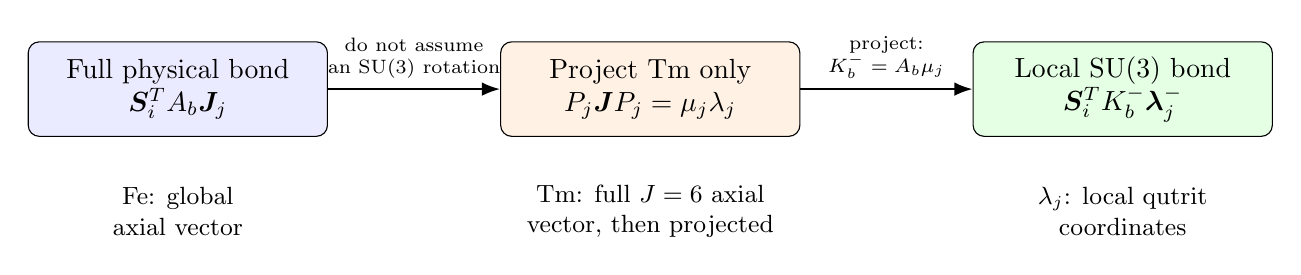
\begin{tikzpicture}[scale=1.0,>=Latex,
  box/.style={draw,rounded corners,align=center,minimum width=3.8cm,minimum height=1.2cm}]
  \node[box,fill=blue!8]    (phys) at (0,0)  {Full physical bond\\$\ve S_i^TA_b\ve J_j$};
  \node[box,fill=orange!10] (proj) at (6,0)  {Project Tm only\\$P_j\ve J P_j=\mu_j\lambda_j$};
  \node[box,fill=green!10]  (k)    at (12,0) {Local SU(3) bond\\$\ve S_i^TK_b^-\lvecminus_j$};
  \draw[->,thick] (phys) -- node[above,align=center,font=\scriptsize]{do not assume\\an SU(3) rotation} (proj);
  \draw[->,thick] (proj) -- node[above,align=center,font=\scriptsize]{project:\\$K_b^-=A_b\mu_j$} (k);
  \node[align=center,font=\small] at (0,-1.55)  {Fe: global\\axial vector};
  \node[align=center,font=\small] at (6,-1.55)  {Tm: full $J=6$ axial\\vector, then projected};
  \node[align=center,font=\small] at (12,-1.55) {$\lambda_j$: local qutrit\\coordinates};
\end{tikzpicture}
\caption{The correct order of operations.  The Tm angular momentum is projected only after the physical symmetry constraints are formulated.}
\end{figure}

\begin{figure}[h]
\centering
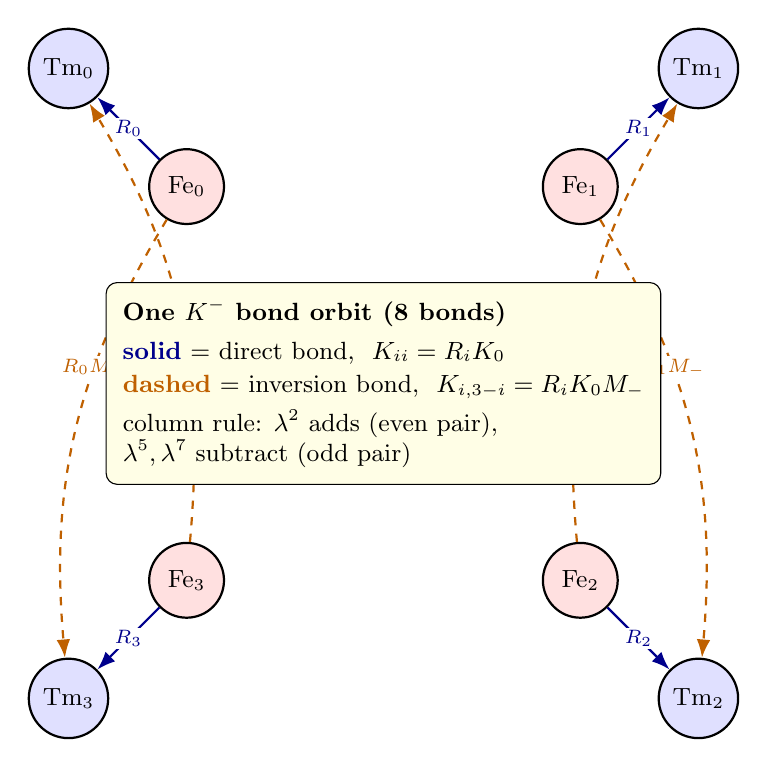
\begin{tikzpicture}[scale=1.0,>=Latex,
  fe/.style={circle,draw,thick,fill=red!12,minimum size=0.95cm,font=\small},
  tm/.style={circle,draw,thick,fill=blue!12,minimum size=0.95cm,font=\small},
  direct/.style={->,thick,blue!55!black},
  inv/.style={->,thick,dashed,orange!75!black}]
  % Fe square (inner), Tm offset outward (outer)
  \node[fe] (F0) at (0,0)    {$\Fe_0$};
  \node[fe] (F1) at (5,0)    {$\Fe_1$};
  \node[fe] (F2) at (5,-5)   {$\Fe_2$};
  \node[fe] (F3) at (0,-5)   {$\Fe_3$};
  \node[tm] (T0) at (-1.5,1.5)  {$\Tm_0$};
  \node[tm] (T1) at (6.5,1.5)   {$\Tm_1$};
  \node[tm] (T2) at (6.5,-6.5)  {$\Tm_2$};
  \node[tm] (T3) at (-1.5,-6.5) {$\Tm_3$};
  % direct (proper-coset) bonds: solid
  \draw[direct] (F0) -- node[midway,fill=white,inner sep=1pt,font=\scriptsize]{$R_0$} (T0);
  \draw[direct] (F1) -- node[midway,fill=white,inner sep=1pt,font=\scriptsize]{$R_1$} (T1);
  \draw[direct] (F2) -- node[midway,fill=white,inner sep=1pt,font=\scriptsize]{$R_2$} (T2);
  \draw[direct] (F3) -- node[midway,fill=white,inner sep=1pt,font=\scriptsize]{$R_3$} (T3);
  % inversion bonds: dashed, run along the outside
  \draw[inv] (F0) to[bend right=18] node[pos=0.35,fill=white,inner sep=1pt,font=\scriptsize]{$R_0M_-$} (T3);
  \draw[inv] (F1) to[bend left=18]  node[pos=0.35,fill=white,inner sep=1pt,font=\scriptsize]{$R_1M_-$} (T2);
  \draw[inv] (F2) to[bend left=18]  node[pos=0.35,fill=white,inner sep=1pt,font=\scriptsize]{$R_2M_-$} (T1);
  \draw[inv] (F3) to[bend right=18] node[pos=0.35,fill=white,inner sep=1pt,font=\scriptsize]{$R_3M_-$} (T0);
  % legend
  \node[draw,rounded corners,align=left,font=\small,fill=yellow!10,inner sep=6pt]
    at (2.5,-2.5)
    {\textbf{One $K^-$ bond orbit (8 bonds)}\\[3pt]
     \textcolor{blue!55!black}{\textbf{solid}} = direct bond,\ \ $K_{ii}=R_iK_0$\\[1pt]
     \textcolor{orange!75!black}{\textbf{dashed}} = inversion bond,\ \ $K_{i,3-i}=R_iK_0M_-$\\[3pt]
     column rule: $\lambda^2$ adds (even pair),\\
     $\lambda^{5},\lambda^{7}$ subtract (odd pair)};
\end{tikzpicture}
\caption{One transported-gauge $K^-$ orbit.  Fe sites (red) sit on inversion
centres; Tm sites (blue) are exchanged in pairs by inversion
($\Tm_0\!\leftrightarrow\!\Tm_3$, $\Tm_1\!\leftrightarrow\!\Tm_2$).  Each Fe
participates in one \emph{direct} bond (solid, coefficient $R_iK_0$) to its own
Tm and one \emph{inversion} bond (dashed, coefficient $R_iK_0M_-$) to the
partner Tm.  Summing the orbit gives the even/odd column rule of
\eqref{eq:orbit-formula}.}
\label{fig:orbit-schematic}
\end{figure}

% =====================================================================
\section{Modeling the 2DCS cross peak: what must a vertex do?}
\label{sec:mechanism}
% =====================================================================

The earlier sections fixed the \emph{form} of every symmetry-allowed Fe--Tm
coupling.  We now ask the sharp dynamical question: which of them can actually
produce the measured $(q_{\mathrm{AFM}},E_{12})$ 2DCS cross peak?  The strategy
is two-step.  First we reduce the whole experiment to a \emph{single} sharp
requirement on an effective Tm force (this section).  Then we test each
candidate coupling against it as a Feynman-diagram catalogue
(\cref{sec:catalog}).  The experimental context is third-order magnetic-dipole
THz 2DCS of orthoferrite magnons~\cite{Lu2017}; the language is standard
nonlinear response theory~\cite{Mukamel}.

\subsection{The observable and $M_{\rm NL}$, precisely}

Two collinear THz pulses give the total drive $B(t)=B_A(t+\tau)+B_B(t)$.  The
detected magnetization is a functional of that field; expand it in powers of
the drive,
\begin{equation}
  M[B]=\sum_{n\ge1}M^{(n)}[\underbrace{B,\dots,B}_{n}].
\end{equation}
With $M_A\equiv M[B_A]$, $M_B\equiv M[B_B]$, $M_{AB}\equiv M[B_A+B_B]$, the
isolated nonlinear signal is
\begin{equation}
  \boxed{\,M_{\rm NL}(t,\tau)=M_{AB}-M_A-M_B\,.}
\end{equation}
Order by order, $M^{(n)}[B_A+B_B]-M^{(n)}[B_A]-M^{(n)}[B_B]$ keeps only the
\emph{mixed} terms, those with at least one factor of each pulse:
\begin{align}
  n=1:&\quad 0 \quad(\text{linear, no mixed term}),\\
  n=2:&\quad 2\,M^{(2)}[B_A,B_B] \quad(\chi^{(2)}\text{-type},\ \propto B_AB_B),\\
  n=3:&\quad M^{(3)}\ \text{mixed} \quad(\chi^{(3)}\text{-type},\ B_A^2B_B+B_AB_B^2).
\end{align}
So $M_{\rm NL}$ is purely nonlinear and starts at second order; the $n=1$ piece
cancels identically.  For magnetic-dipole driving in a centrosymmetric magnet
the leading robust contribution is third order~\cite{Lu2017}.  The detected
quantity at the target is the Tm $c$-axis dipole, $m_z^{\Tm}\propto\lambda^2$,
so the object of interest is $M_{\rm NL}^{\lambda^2}(t,\tau)$, whose 2D
transform should peak at $(\omega_\tau,\omega_t)=(q_{\mathrm{AFM}},E_{12})$.

\subsection{The detection channel: only $\lambda^2$ is bright}

In the $E_{12}$ block the coherence is carried by $\lambda^1=\mathrm{Re}\ket1\bra2$
and $\lambda^2=\mathrm{Im}\ket1\bra2$, both oscillating at $\omega_{12}=E_{12}$,
while $\lambda^3$ is the population imbalance.  From \eqref{eq:mu0} the radiated
moment is
\begin{equation}
  m_z^{\Tm}\propto P_jJ_zP_j=5.264\,\lambda^2,
\end{equation}
so \emph{only $\lambda^2$ is magnetically bright}.  The onsite Hamiltonian
$H_{\Tm,0}\supset-\tfrac{\Delta_{12}}{2}\lambda^3$ generates, through
$[\lambda^3,\lambda^1]=2i\lambda^2$, the planar precession
\begin{equation}
  \dot\lambda^1=-\Delta_{12}\,\lambda^2,\qquad
  \dot\lambda^2=+\Delta_{12}\,\lambda^1 .
\end{equation}
A force on \emph{either} $\lambda^1$ or $\lambda^2$ therefore launches the same
ring at $\omega_{12}$.  We may treat the Tm $E_{12}$ sector as a single driven
oscillator,
\begin{equation}
  \lambda^2(t)=\int_0^t\sin\!\big[\omega_{12}(t-t')\big]\,h^1(t')\,dt',
  \label{eq:tm-osc}
\end{equation}
driven by the effective transverse field $h^1(t)$ that a conversion vertex
exerts on $\lambda^1$.

\subsection{Reframing to a sharp question}

Equation~\eqref{eq:tm-osc} factorizes the 2D map.  The \emph{detection}-axis
($t$) structure is fixed entirely by the Tm pole at $E_{12}$: an impulsive
step force gives a $1-\cos\omega_{12}t$ ring, a delta kick gives a
$\sin\omega_{12}t$ ring.  All the \emph{delay}-axis ($\tau$) information---in
particular whether the peak sits at $\omega_\tau=q_{\mathrm{AFM}}$---lives in the
$\tau$-dependence of $h^1(t,\tau)$.  Hence the entire experiment collapses to
one question:

\begin{keybox}[title={The sharp question}]
A coupling produces the $(q_{\mathrm{AFM}},E_{12})$ cross peak \emph{iff} the
effective Tm force it generates,
\begin{equation}
  M_{\rm NL}^{\lambda^2}(\tau,t)\;\propto\;f(\omega_q\tau)\,\big[1-\cos\omega_{12}t\big],
\end{equation}
has $f$ \emph{oscillating at $\omega_q=q_{\mathrm{AFM}}$}.  Equivalently, the
force $h^1(t,\tau)$ on the bright $\lambda^1$ channel must be (i) nonzero by
symmetry, (ii) able to reach $\lambda^1/\lambda^2$, and (iii) carry an $\omega_q$
modulation along the delay $\tau$.
\end{keybox}

Everything below is the evaluation of $h^1(t,\tau)$ for each candidate vertex.

\subsection{Feynman rules: fields, charges, and the vertex requirement}

We treat the problem as a tree-level field theory.  The propagating ``fields''
(internal/external lines) are
\begin{center}
\renewcommand{\arraystretch}{1.25}
\begin{tabular}{lll}
\toprule
line & object & properties \\
\midrule
Fe magnon & $\delta S_\alpha$ & pole at $\omega_q$; time-odd; the pump excites $\delta S_y$ \\
Tm qutrit & $\lambda^a$ & poles at CEF gaps; $\lambda^-\!=\!\{2,5,7\}$ (T-odd), $\lambda^+\!=\!\{1,3,4,6,8\}$ (T-even) \\
B-photon & $B_\eta(t)$ & external; time-odd, axial \\
E-photon & $E_\eta(t)$ & external; time-even, polar \\
\bottomrule
\end{tabular}
\end{center}
Every Fe magnon line is born from a pulse through the Zeeman source
$g_{\Fe}\mu_B\,\ve B\!\cdot\!\ve S$, so each external Fe leg costs one factor of
the drive.  Three ``charges'' are conserved at every vertex:
\begin{center}
\renewcommand{\arraystretch}{1.3}
\begin{tabular}{ll}
\toprule
charge & rule at a vertex \\
\midrule
energy $\omega$ & a static vertex conserves it $\Rightarrow$ connects only equal frequencies; an external leg injects $\hbar\omega_{\rm drive}$ \\
$\mathcal T$-parity & each term is time-even: $\lambda^-$ needs an \emph{odd} number of T-odd legs $(S,B)$; $\lambda^+$ an \emph{even} number \\
irrep $\Gamma$ & $\Gamma(\text{legs})\otimes\Gamma(\lambda)\supset\Gamma_1$; the orbit sign sums of \eqref{eq:orbit-formula} are this projector \\
\bottomrule
\end{tabular}
\end{center}
Detection and the $M_{\rm NL}$ subtraction add two more bookkeeping rules: the
vertex must reach $\lambda^1/\lambda^2$, and the diagram must attach at least
one leg to each pulse.  Collecting, a successful cross-peak vertex must pass all
six tests:

\begin{keybox}[title={Scorecard R1--R6}]
\begin{description}
\item[R1 (detection)] reaches $\lambda^1/\lambda^2$ (the $E_{12}$ block).
\item[R2 (drive)] is sourced by the pumped $\delta S_y$ magnon.
\item[R3 (parity)] is $\mathcal T$-even, which fixes the $\lambda^\pm$ sector.
\item[R4 (irrep)] is $\Gamma_1$-allowed for the $\Gamma_2/q_{\mathrm{AFM}}$ geometry.
\item[R5 (energy)] can carry the $0.9\!\to\!0.5\,$THz mismatch---needs $\ge2$ non-$\lambda$ legs (two magnons, or one magnon $+$ one photon).
\item[R6 ($M_{\rm NL}$)] involves both pulses.
\end{description}
\end{keybox}

% =====================================================================
\section{The vertex catalogue: a Feynman diagram for each coupling}
\label{sec:catalog}
% =====================================================================

We now write each candidate as an interaction vertex---a term in $H$ with a
coupling constant and a fixed set of legs---draw its tree diagram for the 2DCS
process, and score it against R1--R6.  In every diagram time runs left to
right: a red solid line is an Fe magnon ($\omega_q$), a blue dashed line a Tm
coherence, a wavy arrow an external-field interaction (one pulse); a filled dot
is a field-gated bilinear vertex, a filled square a two-spin vertex.  The boxed
expression above each diagram is the vertex itself.

\subsection{$K^-$: the static bilinear (fails R3/R4/R5)}

\begin{equation}
  \boxed{\;H_{K^-}=K^-_{a\alpha}\,S_\alpha\,\lambda^a,\qquad a\in\{2,5,7\}\;}
  \qquad[\,\text{1 Fe (odd)}+\text{1 Tm}^-\text{(odd)};\ \mathcal T\text{-even};\ \text{no spare leg}\,]
\end{equation}
This is a two-point Fe--Tm vertex; the only process it generates is a single
Fe$\to$Tm line conversion (\cref{fig:vx-kminus}).  It fails in three independent
ways:
\begin{enumerate}
\item \textbf{(R5, linear).}  $K^-$ is linear in $S$, so it adds to the
\emph{quadratic} Hamiltonian---it is a basis rotation among the (harmonic) Fe
and Tm normal modes.  Coupled harmonic oscillators are diagonalizable and their
2D spectrum has \emph{diagonal peaks only}.  A single bilinear hop cannot
transport a $0.9\,$THz coherence into a $0.5\,$THz one: a static vertex
conserves energy, so it can only connect degenerate modes, i.e.\ it
\emph{hybridizes} rather than \emph{converts}.  The lone-pulse hop is in any
case removed by the $M_{\rm NL}$ subtraction (R6).
\item \textbf{(R4, $\Gamma_1$).}  Even the static torque vanishes: for the
patterns $F_x$, $G_z$ and the pumped $\delta S_y$ the four-site orbit sums give
$[0,0,0,0]$ for every channel except $K^-_{2y}\!\to\![8,8,8,8]$
(\cref{sec:numerical}).  All channels but $2y$ are $\Gamma_1$-forbidden.
\item \textbf{(reorientation).}  The one $\Gamma_1$-allowed channel, $K^-_{2y}$,
is a transverse molecular field on the order parameter; it reorients
$\Gamma_2\!\to\!G_y$ before any spectroscopic regime (lost between $0.085$ and
$0.090\,$meV).  It is not a perturbative vertex.
\end{enumerate}

\begin{figure}[h]
\centering
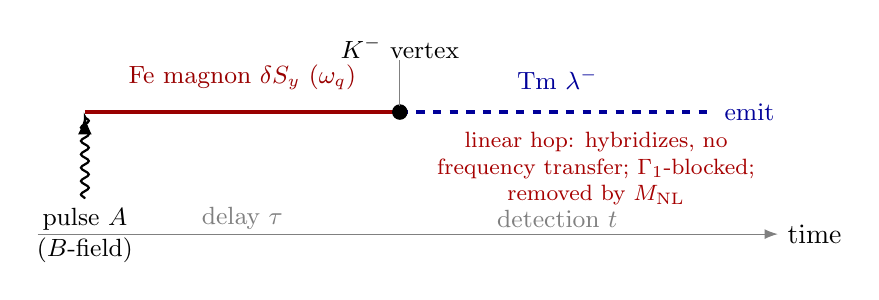
\begin{tikzpicture}[>=Latex,
  fe/.style={very thick,red!60!black},
  tm/.style={very thick,dashed,blue!60!black},
  photon/.style={->,thick,decorate,decoration={snake,amplitude=0.5mm,segment length=1.7mm}}]
  \draw[fe] (0,0)--(4,0);
  \draw[tm] (4,0)--(8,0);
  \filldraw[black] (4,0) circle (2.6pt);
  \draw[gray,thin] (4,0.08)--(4,0.66);
  \node[black,font=\small] at (4,0.82) {$K^-$ vertex};
  \node[above,red!60!black,font=\small]  at (2,0.16) {Fe magnon $\delta S_y$ ($\omega_q$)};
  \node[above,blue!60!black,font=\small] at (6,0.16) {Tm $\lambda^-$};
  \node[right,blue!60!black,font=\small] at (8,0) {emit};
  \draw[photon] (0,-1.1)--(0,-0.05);
  \node[below,align=center,font=\small] at (0,-1.1) {pulse $A$\\($B$-field)};
  \node[align=center,red!65!black,font=\footnotesize,anchor=west] at (4.35,-0.72)
    {linear hop: hybridizes, no\\ frequency transfer; $\Gamma_1$-blocked;\\ removed by $M_{\rm NL}$};
  \draw[->,gray] (-0.6,-1.55) -- (8.8,-1.55) node[right,black]{time};
  \node[gray,font=\small] at (2,-1.35) {delay $\tau$};
  \node[gray,font=\small] at (6,-1.35) {detection $t$};
\end{tikzpicture}
\caption{$K^-$ (fails).  A single Fe leg converts to a single $\lambda^-$ leg---a
linear hop.  It only hybridizes the modes, the conversion matrix element is
$\Gamma_1$-cancelled, and the lone-pulse path is subtracted in $M_{\rm NL}$.}
\label{fig:vx-kminus}
\end{figure}

\begin{keybox}[title={The longitudinal temptation, and why it is still trapped}]
One might smuggle in two-magnon content through the \emph{longitudinal}
component $S_z=S_z^{(0)}-\delta S_\perp^2/2S_z^{(0)}$: a bilinear $K\,S_z\lambda$
does contain $\delta S_y^2\,\lambda$.  But $S_z$ is time-odd, so $K\,S_z\lambda$
must place $\lambda$ in $\lambda^-$---it \emph{is} $K^-_{2z,5z,7z}$.  The hidden
$\delta S_z$ carries the $G_z$ sublattice sign pattern, so it cancels in the
\emph{same} orbit sum as the static $G_z$ torque.  The two-magnon signal is real
but parity-trapped in $\lambda^-$ and $\Gamma_1$-cancelled---confirmed by the
full nonlinear $K^-_{2z}$ run (which contains the spin-length constraint) being
dark to $10^{-15}$ even at $2.0\,$meV (\cref{sec:numerical}).  To reach
$\lambda^1$ the \emph{same} $\delta S_y^2$ content must be carried by a
$\mathcal T$-even Fe operator: two spin legs ($W$) or a field leg ($\kappa^B$).
\end{keybox}

\subsection{$ESJ$: electric-field-assisted (works, but wrong target---fails R1)}

\begin{equation}
  \boxed{\;H_{ESJ}(t)=\kappa^E_{a\alpha\eta}\,E_\eta(t)\,S_\alpha\,\lambda^a,\qquad a\in\{2,5,7\}\;}
  \quad[\,\text{1 E (even)}+\text{1 Fe (odd)}+\text{1 Tm}^-\text{(odd)};\ \mathcal T\text{-even}\,]
\end{equation}
A genuine three-point vertex (\cref{fig:vx-esj}): pulse $A$'s magnetic field
makes the Fe coherence, pulse $B$'s \emph{electric} field enters at the vertex,
and the $E$-photon supplies the energy mismatch (R5 $\checkmark$, R6
$\checkmark$, R2 $\checkmark$).  But it feeds $\lambda^-$, and the surviving
inversion-even combination under $-M_-$ is $\lambda^5,\lambda^7$---the $E_{13}$
and $E_{23}$ coherences, \emph{not} $E_{12}$.  So $ESJ$ produces real cross peaks
at $(q_{\mathrm{AFM}},E_{13})$ and $(q_{\mathrm{AFM}},E_{23})$, but lands on the
wrong readout for $E_{12}$ (fails R1).

\begin{figure}[h]
\centering
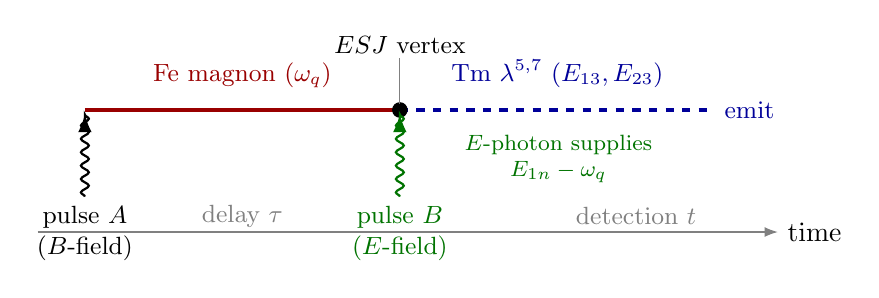
\begin{tikzpicture}[>=Latex,
  fe/.style={very thick,red!60!black},
  tm/.style={very thick,dashed,blue!60!black},
  photon/.style={->,thick,decorate,decoration={snake,amplitude=0.5mm,segment length=1.7mm}}]
  \draw[fe] (0,0)--(4,0);
  \draw[tm] (4,0)--(8,0);
  \filldraw[black] (4,0) circle (2.6pt);
  \draw[gray,thin] (4,0.08)--(4,0.66);
  \node[black,font=\small] at (4,0.82) {$ESJ$ vertex};
  \node[above,red!60!black,font=\small]  at (2,0.16) {Fe magnon ($\omega_q$)};
  \node[above,blue!60!black,font=\small] at (6,0.16) {Tm $\lambda^{5,7}$ ($E_{13},E_{23}$)};
  \node[right,blue!60!black,font=\small] at (8,0) {emit};
  \draw[photon] (0,-1.1)--(0,-0.05);
  \node[below,align=center,font=\small] at (0,-1.1) {pulse $A$\\($B$-field)};
  \draw[photon,green!45!black] (4,-1.1)--(4,-0.05);
  \node[below,align=center,green!45!black,font=\small] at (4,-1.1) {pulse $B$\\($E$-field)};
  \node[align=center,green!45!black,font=\footnotesize,anchor=west] at (4.7,-0.62)
    {$E$-photon supplies\\$E_{1n}-\omega_q$};
  \draw[->,gray] (-0.6,-1.55) -- (8.8,-1.55) node[right,black]{time};
  \node[gray,font=\small] at (2,-1.35) {delay $\tau$};
  \node[gray,font=\small] at (7,-1.35) {detection $t$};
\end{tikzpicture}
\caption{$ESJ$ (works, wrong target).  A clean three-point vertex; the
$E$-photon carries the energy mismatch.  But it feeds $\lambda^{5,7}$, so it
lights up $E_{13}/E_{23}$, not the $E_{12}$ target.}
\label{fig:vx-esj}
\end{figure}

\subsection{$W=SS\lambda$: the two-magnon vertex (passes all---the winner)}

\begin{equation}
  \boxed{\;H_W=W^a_{\alpha\beta}\,S_\alpha S_\beta\,\lambda^a,\qquad a\in\{1,3,4,6,8\}\;}
  \quad[\,\text{2 Fe (odd$\times$odd$=$even)}+\text{1 Tm}^+\text{(even)};\ \mathcal T\text{-even};\ \text{no photon}\,]
\end{equation}
For the pump geometry the active term is $W^{yy}_1\,S_y^2\,\lambda^1$ (R2: two
$y$-magnon legs; R1: $\lambda^1$).  This is a three-point vertex with \emph{two}
Fe legs, one sourced by each pulse (R6); see \cref{fig:vx-w}.  The vertex feels
$h^1(t)=W^{yy}_1\,S_y(t)^2$ with
$S_y(t)=A[\sin\omega_q(t+\tau)+\theta(t)\sin\omega_q t]$.  The only term
surviving $M_{\rm NL}$ is the two-pulse cross product $2S_y^aS_y^b$, which
\emph{rectifies}:
\begin{equation}
  h^1_{\rm NL}(t,\tau)=W^{yy}_1A^2\big[\underbrace{\cos\omega_q\tau}_{\text{difference}}
  -\underbrace{\cos\omega_q(2t+\tau)}_{\text{sum}}\big]\theta(t).
\end{equation}
The difference term is a $t$-independent step, born at the probe, which through
\eqref{eq:tm-osc} launches the $1-\cos\omega_{12}t$ ring.  Hence
\begin{equation}
  \boxed{\,M_{\rm NL}^{W}(\tau,t)\;\propto\;W^{yy}_1A^2\,\cos(\omega_q\tau)\,
  \big[1-\cos\omega_{12}t\big]\,.}
\end{equation}
This is exactly the sharp-question form: it factorizes, oscillating at $\omega_q$
along $\tau$ and at $\omega_{12}$ along $t$ (R3 with the delay modulation at
$\omega_q$), giving a single sharp peak at $(q_{\mathrm{AFM}},E_{12})$ with no
diagonal partner (the $2\omega_q$ ``sum'' companion is off-resonant).  The
simulated $\lambda^2$ map has its rank-1 maximum exactly here, amplitude $51.0$,
SNR $117$, the $(E_{12},E_{12})$ diagonal $\sim\!50\times$
weaker~\cite{HOreport}; $yy$ beats $xx$ by $\sim\!600\times$ (R2: $S_x$ is the
static $F_x$, barely fluctuating).

\emph{Where the $E_{12}$ energy comes from (verified).}  Since $\delta S_y^2$
contains only $0$ and $2\omega_q$, a static three-leg vertex between \emph{free}
modes could never emit at $\omega_{12}$.  The resolution is that the magnon legs
are pulsed envelopes, not free modes: the rectified cross term is a
\emph{suddenly switched-on step}, and a step carries spectral weight at all
frequencies in its edge, $\propto e^{-\omega_{12}^2\sigma^2/2}$ for rise time
$\sigma$.  Quantum mechanically this is an intra-pulse difference-frequency
(impulsive-Raman) process: the $E_{12}$ quantum is drawn from the \emph{pulse
bandwidth}, while the magnon pair carries only the phase memory
$\cos\omega_q\tau$.  The mechanism is displacive and therefore requires
nonadiabaticity---a falsifiable statement verified directly
(\cref{sec:validation}): stretching the pulse from $\sigma=0.25$ to $1.0$ at
fixed amplitude collapses the peak by $4.5$ decades
($51.7\to1.7\times10^{-3}$), the adiabatic suppression the step picture
demands, while switching the direct Tm drive off changes the peak by
$<10^{-4}$ relative (pure-$W$ origin).  The same sweep resolves the second Fe
leg: for impulsive pulses it is the resonant probe magnon (peak $\propto
A^2$); for longer pulses it crosses over to the \emph{field-following
quasistatic tilt} $\delta S^{\rm qs}(t)\propto B(t)$ (peak $\propto A^1$)---both
$W$-mediated, same peak location.  The quasistatic leg also enables the
\emph{reverse} conversion
$\lambda^{1,2}(\tau)\times\delta S^{\rm qs}(\text{pulse }B)\to
q_{\mathrm{AFM}}$, an $(E_{12},q_{\mathrm{AFM}})$ feature in the Fe channel
whenever a first-order $E_{12}$ delay coherence exists
(\cref{sec:fullscenario}).

\begin{figure}[h]
\centering
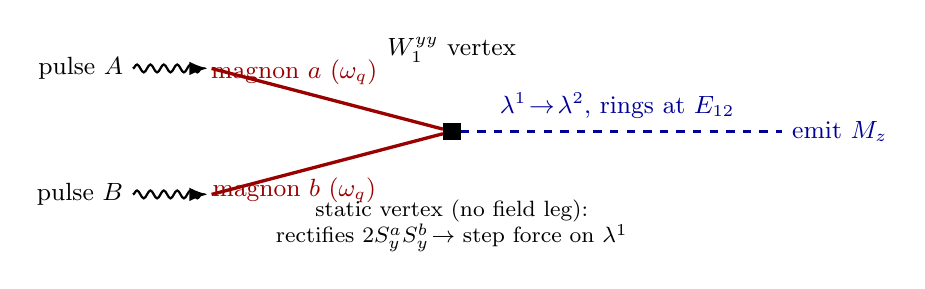
\begin{tikzpicture}[>=Latex,
  fe/.style={very thick,red!60!black},
  tm/.style={very thick,dashed,blue!60!black},
  photon/.style={->,thick,decorate,decoration={snake,amplitude=0.5mm,segment length=1.7mm}}]
  \node[draw,fill=black,rectangle,minimum size=6pt,inner sep=0pt] (W) at (3.5,0) {};
  \node[font=\small] at (3.5,1.04) {$W^{yy}_1$ vertex};
  \draw[fe] (0.45,0.8) -- (W);
  \draw[fe] (0.45,-0.8) -- (W);
  \node[red!60!black,font=\small] at (1.5,0.75) {magnon $a$ ($\omega_q$)};
  \node[red!60!black,font=\small] at (1.5,-0.75) {magnon $b$ ($\omega_q$)};
  \draw[photon] (-0.55,0.8)--(0.4,0.8);  \node[left,font=\small] at (-0.55,0.8){pulse $A$};
  \draw[photon] (-0.55,-0.8)--(0.4,-0.8);\node[left,font=\small] at (-0.55,-0.8){pulse $B$};
  \draw[tm] (W) -- (7.7,0);
  \node[blue!60!black,font=\small,above] at (5.6,0.04) {$\lambda^1\!\to\!\lambda^2$, rings at $E_{12}$};
  \node[blue!60!black,font=\small,right] at (7.7,0) {emit $M_z$};
  \node[align=center,font=\footnotesize] at (3.5,-1.2)
    {static vertex (no field leg):\\ rectifies $2S_y^aS_y^b\!\to$ step force on $\lambda^1$};
\end{tikzpicture}
\caption{$W^{yy}_1$ (winner).  Each pulse makes one $\delta S_y$ magnon; the two
converge on the time-independent $S_y^2\lambda^1$ vertex (square), whose
two-pulse cross term rectifies to a step force that launches the
$\lambda^1\!\to\!\lambda^2$ ring at $E_{12}$.  The response factorizes,
$\cos(\omega_q\tau)[1-\cos\omega_{12}t]$, giving the clean rank-1 cross peak.}
\label{fig:vx-w}
\end{figure}

\subsection{$\kappa^B=BS\lambda$: magnetic-field-assisted (passes, but noisy)}

\begin{equation}
  \boxed{\;H_{\kappa B}(t)=\kappa^B_{a\alpha\eta}\,B_\eta(t)\,S_\alpha\,\lambda^a,\qquad a\in\{1,3,4,6,8\}\;}
  \quad[\,\text{1 B (odd)}+\text{1 Fe (odd)}+\text{1 Tm}^+\text{(even)};\ \mathcal T\text{-even}\,]
\end{equation}
The active term is $\kappa^B_{1y}\,B_y\,S_y\,\lambda^1$.  A three-point vertex
with one $B$-photon, one Fe leg and one $\lambda^+$ leg (\cref{fig:vx-kappab});
the $B$-photon supplies the mismatch (R5).  It is field-gated:
$h^1(t)=\kappa^B_{1y}\,\mathcal B_y(t)\,S_y(t)$ with $\mathcal B_y(t)$ sharply
localized at the pulses.  At the probe $t=0$, $S_y(0)=A\sin\omega_q\tau$, so the
kick $\propto\sin\omega_q\tau$ launches the same ring,
\begin{equation}
  \boxed{\,M_{\rm NL}^{\kappa B}(\tau,t)\;\propto\;\kappa^B_{1y}\,\sin(\omega_q\tau)\,
  \big[1-\cos\omega_{12}t\big]\,,}
\end{equation}
again on target (R1--R6 $\checkmark$).  This is the $BS\lambda^+$ analogue of
$ESJ$, feeding $\lambda^1$ instead of $\lambda^{5,7}$.  The price: the same gated
vertex also dumps each pulse's \emph{local} Fe response into Tm at both pulse
times, generating a strong $(E_{12},E_{12})$ diagonal and a $(0,E_{12})$
background that dominate the bare cross peak (the on-target maximum is genuine
but only rank-3 at zero carrier).  A carrier resonant with a Tm transition
cleans this up---a sweep amplifies the target $\sim\!13\times$ at
$\Omega_B=0.70\,$THz ($E_{23}$)~\cite{HOreport}.  The definitive resolution,
however, is not a carrier but the \emph{polarization} of the gate: the physical
vertex is gated by the lab-frame field component $B_\eta(t)$, and its dominant
symmetry slice is $z$-gated, so in the $H\!\parallel\!a$ geometry ($B_z=0$)
$\kappa^B$ is identically silent and its noise never appears.  Its proper home
is the $H\!\parallel\!c$ geometry, where it produces the measured
$(E_{12},q_{\mathrm{AFM}})$ cross peak; see
\cref{sec:fullscenario,fig:vx-kb2}.

\begin{figure}[h]
\centering
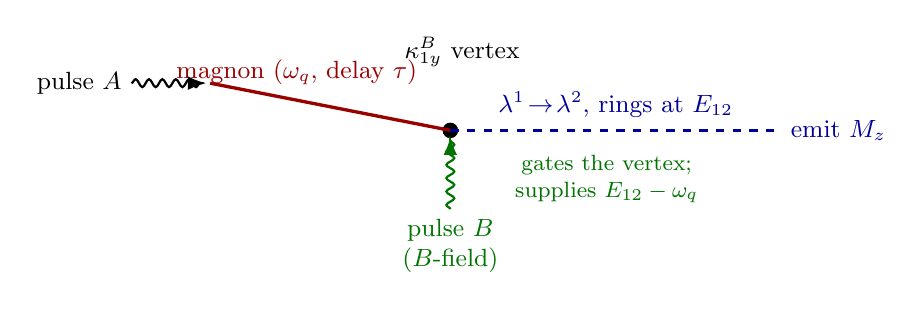
\begin{tikzpicture}[>=Latex,
  fe/.style={very thick,red!60!black},
  tm/.style={very thick,dashed,blue!60!black},
  photon/.style={->,thick,decorate,decoration={snake,amplitude=0.5mm,segment length=1.7mm}}]
  \filldraw[black] (3.5,0) circle (2.6pt);
  \node[font=\small] at (3.65,1.0) {$\kappa^B_{1y}$ vertex};
  \draw[fe] (0.45,0.6) -- (3.5,0);
  \node[red!60!black,font=\small] at (1.55,0.74) {magnon ($\omega_q$, delay $\tau$)};
  \draw[photon] (-0.55,0.6)--(0.4,0.6); \node[left,font=\small] at (-0.55,0.6){pulse $A$};
  \draw[photon,green!45!black] (3.5,-1.0)--(3.5,-0.08);
  \node[below,align=center,green!45!black,font=\small] at (3.5,-1.0) {pulse $B$\\($B$-field)};
  \node[align=center,green!45!black,font=\footnotesize,anchor=west] at (4.2,-0.62)
    {gates the vertex;\\ supplies $E_{12}-\omega_q$};
  \draw[tm] (3.5,0) -- (7.7,0);
  \node[blue!60!black,font=\small,above] at (5.6,0.04) {$\lambda^1\!\to\!\lambda^2$, rings at $E_{12}$};
  \node[blue!60!black,font=\small,right] at (7.7,0) {emit $M_z$};
\end{tikzpicture}
\caption{$\kappa^B_{1y}$ (works, noisy).  One magnon from pulse $A$ meets the
magnetic field of pulse $B$ at the $S_y\lambda^1$ vertex; the $B$-photon gates
the conversion and carries the mismatch.  Same $\lambda^1\!\to\!\lambda^2$
readout as $W^{yy}_1$, but it also feeds the $(E_{12},E_{12})$ diagonal and a
$(0,E_{12})$ background, so it needs a resonant carrier to be a robust target.}
\label{fig:vx-kappab}
\end{figure}

\subsection{Scorecard}

\begin{center}
\renewcommand{\arraystretch}{1.3}
\begin{tabular}{lccccccl}
\toprule
vertex & term & legs & sector & R1 & R2 & R3/4/5 & verdict \\
\midrule
$K^-$        & $S\lambda^-$   & $1\Fe{+}1\Tm^-$        & $\lambda^-$ & $\times$ & --- & $\times$ & hybridizes / $\Gamma_1$-blocked / reorients \\
$ESJ$        & $ES\lambda^-$  & $E{+}\Fe{+}\Tm^-$      & $\lambda^-$ & $\times$ & \checkmark & \checkmark & real, but on $E_{13}/E_{23}$ \\
$W$          & $SS\lambda^+$  & $2\Fe{+}\Tm^+$         & $\lambda^+$ & \checkmark & \checkmark($yy$) & \checkmark & \textbf{winner: rank-1, factorized} \\
$\kappa^B$   & $BS\lambda^+$  & $B{+}\Fe{+}\Tm^+$      & $\lambda^+$ & \checkmark & \checkmark($1y$) & \checkmark & works; $B_z$-gated, geometry 2 \\
\bottomrule
\end{tabular}
\end{center}
The two passes share the same readout, $\lambda^1\!\to\!\lambda^2$ at $E_{12}$,
and differ only in how the Fe motion is fed in: $W$ uses \emph{two} magnon legs
(difference-frequency rectification), $\kappa^B$ uses \emph{one} magnon leg plus
a photon.  Both are the minimal $\mathcal T$-even ways to deliver the
$\delta S_y^2$ two-magnon signal onto the bright $\lambda^1$---the step that
$K^-$, trapped in $\lambda^-$, cannot take.

% =====================================================================
\section{Numerical confirmation}
\label{sec:numerical}
% =====================================================================

The catalogue is confirmed by direct simulation in the calibrated
$1\times1\times1$ mixed TmFeO$_3$ model.  All 2DCS runs use Fe pump
$H\!\parallel x$, $\tau\in[-40,0]$, $t\in[-40,40]$, and step $\Delta t=0.02$
(code units); the Tm sector is not directly pumped unless stated.

\subsection{Static one-at-a-time $K^-$ scan ($0.2\,$meV): the $\Gamma_1$ block}

A static ground-state scan with one $K^-$ component on at a time confirms R4
directly:
\begin{center}
\renewcommand{\arraystretch}{1.15}
\begin{tabular}{lcccc}
\toprule
component & $E/N$ (meV) & Fe order & $(\lambda_2,\lambda_5,\lambda_7)_{\rm uniform}$ & verdict \\
\midrule
baseline & $-42.496758$ & $F_x+G_z$ & $(0,0,0)$ & reference \\
$K^-_{2x}$ & $-42.496758$ & $F_x+G_z$ & $(0,0,0)$ & inert \\
$K^-_{2y}$ & $-43.654818$ & $G_y$ & $(0.888320,0,0)$ & spin reorients \\
$K^-_{2z}$ & $-42.496758$ & $F_x+G_z$ & $(0,0,0)$ & inert \\
$K^-_{5x}$ & $-42.496758$ & $F_x+G_z$ & $(0,0,0)$ & inert \\
$K^-_{5y}$ & $-42.496758$ & $F_x+G_z$ & $(0,0,0)$ & inert \\
$K^-_{5z}$ & $-42.496758$ & $F_x+G_z$ & $(0,0,0)$ & inert \\
$K^-_{7x}$ & $-42.496758$ & $F_x+G_z$ & $(0,0,0)$ & inert \\
$K^-_{7y}$ & $-42.496758$ & $F_x+G_z$ & $(0,0,0)$ & inert \\
$K^-_{7z}$ & $-42.496758$ & $F_x+G_z$ & $(0,0,0)$ & inert \\
\bottomrule
\end{tabular}
\end{center}
Only $K^-_{2y}$ does anything, and it does so by leaving $\Gamma_2$: an adiabatic
ramp keeps $\Gamma_2$ stable through $0.085\,$meV and loses it by $0.090\,$meV,
flipping to $G_y$ with a large uniform $\lambda_2$.  The pattern is the exact
orbit sign algebra ($R_i$ with $M_-=\diag(+1,-1,-1)$):
\begin{align}
  F_x:&\ K^-_{2x},K^-_{5x},K^-_{7x}\to[0,0,0,0], &
  G_z:&\ K^-_{2z},K^-_{5z},K^-_{7z}\to[0,0,0,0], \\
  \delta S_y:&\ K^-_{2y}\to[8,8,8,8], &
  \delta S_y:&\ K^-_{5y},K^-_{7y}\to[0,0,0,0].
\end{align}

\subsection{Fe-pump 2DCS on the inert channels: dark to machine precision}

Running 2DCS on the inert channels (Fe pump only) and extracting the maximum
nonlinear SU(3) amplitude over the $(t,\tau)$ grid confirms R5---these are
dark even with the \emph{full} nonlinear dynamics (hence including the
longitudinal $\delta S_z$ rectification):
\begin{center}
\renewcommand{\arraystretch}{1.15}
\begin{tabular}{lccc}
\toprule
run & $\max|M_{\rm NL}^{\lambda_2}|$ & $\max|M_{\rm NL}^{\lambda_5}|$ & $\max|M_{\rm NL}^{\lambda_7}|$ \\
\midrule
$K^-_{2x}=0.2$ & $6.06\times10^{-18}$ & $0$ & $0$ \\
$K^-_{2x}=1.5$ & $2.96\times10^{-16}$ & $0$ & $0$ \\
$K^-_{2z}=0.2$ & $9.87\times10^{-16}$ & $0$ & $0$ \\
$K^-_{2z}=2.0$ & $6.86\times10^{-15}$ & $0$ & $0$ \\
$K^-_{5y}=0.2$ & $0$ & $0$ & $0$ \\
$K^-_{7y}=0.2$ & $0$ & $0$ & $0$ \\
\bottomrule
\end{tabular}
\end{center}
Up to $K^-_{2x}=1.5\,$meV and $K^-_{2z}=2.0\,$meV the induced $\lambda_2$ is at
machine precision---the bilinear cannot, even nonlinearly, manufacture the
$E_{12}$ coherence.  Adding a direct Tm $H\!\parallel x$ pump on top reproduces
the ordinary Tm response and reveals no hidden $K^-$ channel.  By contrast, the
no-damping scan over the higher-order set isolates exactly $W^{yy}_1$ (rank-1,
$|M_{\rm NL}^{\lambda_2}|=51.0$, SNR $117$) and $\kappa^B_{1y}$ as the on-target
vertices~\cite{HOreport}, precisely the two that pass R1--R6.

% =====================================================================
\section{The full scenario: one Hamiltonian, all measured geometries}
\label{sec:fullscenario}
% =====================================================================

\Cref{sec:catalog} answered the original narrow question---which vertex makes
the $(q_{\mathrm{AFM}},E_{12})$ peak---in a single geometry.  The experiment,
however, provides \emph{three} pulse/detection geometries, and the full data
set is a peak inventory.  This section assembles the validated end-to-end
picture: one fixed Hamiltonian, physical pulses, and a polarization or
selection gate attached to every coupling, such that each geometry
self-selects its own subset of cross peaks with no per-geometry retuning.
Frequencies are quoted in THz,
\begin{equation}
  \omega_F=0.38\ (q_{\mathrm{FM}}),\qquad
  \omega_q=0.90\ (q_{\mathrm{AFM}}),\qquad
  \omega_{12}=0.50,\qquad \omega_{23}=0.70,\qquad
  \omega_{13}=1.20=\omega_{12}+\omega_{23},
\end{equation}
the last identity being the shared-level ladder $1\!\to\!2\!\to\!3$ of the Tm
qutrit.

\subsection{Geometries, pulse composition, and detection channels}
\label{sec:geometries}

A THz pulse propagating along $b$ carries either $(E\!\parallel\!c,
B\!\parallel\!a)$ or $(E\!\parallel\!a, B\!\parallel\!c)$.  Each field
component couples to a fixed set of modes, and each Tm block emits into a
fixed polarization channel through the magnetic dipole matrix
$\mu$ of \eqref{eq:mu0} ($\lambda^2\!\to\!m_z$ via $\mu_{2z}=5.264$;
$\lambda^{5},\lambda^{7}\!\to\!m_x$ via $\mu_{5x}=2.39,\ \mu_{7x}=0.91$):

\begin{center}
\renewcommand{\arraystretch}{1.3}
\small
\begin{tabular}{llll}
\toprule
 & pulse & drives (delay-axis coherences) & detection channels \\
\midrule
$\mathcal G_A$: $H\!\parallel\!a$, $E\!\parallel\!c$
 & $B\!\parallel\!a$ & Fe $q_{\mathrm{AFM}}$ ($\theta{=}0$);\ Tm $\lambda^{5},\lambda^{7}$
 & \emph{cross-pol} ($E\!\parallel\!a\!\leftarrow\!m_z\!\leftarrow\!\lambda^2$): geom.\ 1 \\
 & $E\!\parallel\!c$ & Tm $\lambda^{2}$ ($E_{12}$ $c$-axis dipole)
 & \emph{same-pol} ($E\!\parallel\!c\!\leftarrow\!m_x\!\leftarrow\!\lambda^{5,7}$): geom.\ 3 \\
\midrule
$\mathcal G_B$: $H\!\parallel\!c$, $E\!\parallel\!a$
 & $B\!\parallel\!c$ & Fe $q_{\mathrm{FM}}$ ($\theta{=}90^\circ$);\ Tm $\lambda^{2}$ ($\mu_{2z}$)
 & Fe magnon channel ($F_x$): geom.\ 2 \\
\bottomrule
\end{tabular}
\end{center}

Geometries 1 and 3 are therefore the \emph{same physical run} read in the two
orthogonal analyzer channels; $B\!\parallel\!a$ never reaches $\lambda^2$
($\mu_{2x}=0$), and $B\!\parallel\!c$ never reaches $\lambda^{5,7}$
($\mu_{5z}=\mu_{7z}=0$).  These two zeros of the $\mu$ matrix are the first two
gates of the story.

\subsection{The mode inventory: the physics of every frequency}
\label{sec:modes}

Six frequencies carry the entire 2DCS phenomenology.  For each we state what
oscillates, what sets the frequency, how it is driven, how it radiates, and its
linewidth---these five properties, combined with the vertices of
\cref{sec:couplinglist}, determine every peak in every geometry.

\paragraph{$q_{\mathrm{FM}}$ ($\omega_F=0.38$\,THz): the quasi-ferromagnetic
magnon.}  Precession of the weak net moment $\ve F\!\parallel\!a$ about its
equilibrium; in the simulation it is \emph{uniform} $\delta S_y$ with a
staggered $\delta S_x$ counterpart.  The restoring force is the in-plane
anisotropy (gap $\propto\sqrt{JK}$), making it the softer magnon.
Zeeman-driven only when the field can torque $\ve F$: $\ve B\perp\ve M$, i.e.\
$H\!\parallel\!c$ (the $\theta$ selection rule)---which is why it exists only
in geometry 2.  In $\mathcal G_A$ its emission polarization ($m_y$) is
longitudinal to the propagation, and its nonlinear channel is dark to
$10^{-11}$.  2DCS role: the \emph{delay} coherence of $(\omega_F,\omega_q)$ in
geometry 2.

\paragraph{$q_{\mathrm{AFM}}$ ($\omega_q=0.90$\,THz): the quasi-antiferromagnetic
magnon.}  Oscillation of the N\'eel vector: \emph{staggered} $\delta
S_y,\delta S_z$ with only a small \emph{uniform} $F_x$ projection inherited
from the DM canting.  (Practical corollary, learned the hard way: its
amplitude must be measured on the staggered magnetization; the uniform $\ve M$
is blind to it at linear order.)  Gap set by exchange$\times$anisotropy plus
DM.  Zeeman-driven when $\ve B\!\parallel\!\ve M$ ($H\!\parallel\!a$).  2DCS
roles: delay coherence of $(\omega_q,E_{12})$ [G1] and $(\omega_q,E_{23})$
[G3]; \emph{detection} frequency of both geometry-2 cross peaks (read out
through the uniform $F_x$ projection); the Fe-channel diagonal.

\paragraph{$\omega_{\rm s}$ ($\approx0.1$\,THz): the reorientation soft mode.}
Rigid rotation of $\ve F$ in the $a$--$c$ plane (uniform $S_z$)---the
$\Gamma_2\!\to\!\Gamma_4$ reorientation coordinate.  Soft because
$|K_a-K_c|=0.003$\,meV: the spin-reorientation proximity of TmFeO$_3$
expressed at $T=0$.  It is neither a delay nor a detection frequency of any
listed peak; it appears solely as $\pm\omega_{\rm s}$ amplitude-modulation
sidebands on the strong peaks, carried between sectors by $W$.  Its frequency
is a thermometer of the reorientation, $\omega_{\rm s}(T)\!\to\!0$ at
$T_{\rm SR}$.

\paragraph{$E_{12}$ ($\omega_{12}=0.50$\,THz): the ground-doublet coherence.}
The $\ket1\!\leftrightarrow\!\ket2$ coherence of the Tm qutrit, carried by
$\lambda^1$ (T-even, dark) and $\lambda^2$ (T-odd, magnetically bright:
$m_z=\mu_{2z}\lambda^2$ with $\mu_{2z}=5.264$).  Frequency $=$ the calibrated
CEF splitting $e_1=2.068$\,meV; narrow (long-lived ground-doublet coherence,
$\gamma_{\lambda^{1,2}}\approx0$).  It has \emph{three distinct sources, one
per mechanism class}: $W$-rectification (whenever a magnon is pumped);
$\mu_{2z}B_z$ (geometry B, first order); the exchange-induced
$d^{\rm eff}_zE_z$ (geometry A, first order).  Radiates $m_z$ into the
cross-polarized channel.  2DCS roles: detection frequency of geometry 1; delay
coherence of $(E_{12},\omega_q)$ [G2] and of both geometry-3 transfer peaks.

\paragraph{$E_{23}$ ($\omega_{23}=0.70$\,THz): the dark upper coherence.}
$\ket2\!\leftrightarrow\!\ket3$, carried by $\lambda^{6}$/$\lambda^{7}$;
magnetic $x$-dipole $\mu_{7x}=0.91$ ($m_x\to$ same-pol channel).  It is
first-order \emph{dark from the ground state}---both of its levels are empty,
so $\lambda^{6,7}$ acting on $\ket1$ gives exactly zero---hence every
$\omega_t=E_{23}$ feature is necessarily a conversion product, never a pump
artifact.  Broad: it involves the short-lived level 3
($\gamma_{\lambda^{4\ldots7}}=0.15$\,meV).  2DCS roles: detection frequency of
$(E_{12},E_{23})$ and $(\omega_q,E_{23})$ [G3].

\paragraph{$E_{13}$ ($\omega_{13}=1.20$\,THz): the bright upper coherence.}
$\ket1\!\leftrightarrow\!\ket3$, carried by $\lambda^{4}$/$\lambda^{5}$; the
strong magnetic $x$-dipole $\mu_{5x}=2.39$ ($m_x\to$ same-pol).  Bright from
the ground state and therefore directly pumped by $B\!\parallel\!a$---but its
\emph{delay} coherence is erased by the level-3 linewidth, so it survives only
as a detection frequency.  The exact ladder identity
$\omega_{13}=\omega_{12}+\omega_{23}$ closes the qutrit transfer algebra:
$f_{abc}$ rotates $\rho_{12}$ into $\rho_{13}$ or $\rho_{32}$ with no energy
left over.  2DCS roles: detection frequency of $(E_{12},E_{13})$ and of the
faint shared-level partner $(E_{23},E_{13})$.

\begin{center}
\renewcommand{\arraystretch}{1.3}
\footnotesize
\begin{tabular}{lllllll}
\toprule
mode & THz & carrier & driven by & radiates & width & 2DCS roles \\
\midrule
$q_{\mathrm{FM}}$ & $0.38$ & unif.\ $\delta S_y$ & $B\perp M$ ($\mathcal G_B$) & (longitudinal) & narrow & delay [G2] \\
$q_{\mathrm{AFM}}$ & $0.90$ & stag.\ $\delta S_{y,z}$ $(+F_x)$ & $B\parallel M$ ($\mathcal G_A$) & $F_x\!\to$ same-pol & narrow & delay [G1,G3]; det.\ [G2] \\
$\omega_{\rm s}$ & $\sim0.1$ & unif.\ $S_z$ ($a$--$c$) & nonlinear only & --- & soft & sidebands only \\
$E_{12}$ & $0.50$ & $\lambda^{1,2}$ & $W$; $\mu_{2z}B_z$; $d^{\rm eff}_zE_z$ & $m_z\!\to$ cross-pol & narrow & det.\ [G1]; delay [G2,G3] \\
$E_{23}$ & $0.70$ & $\lambda^{6,7}$ & dark (conversion only) & $m_x\!\to$ same-pol & $\gamma$ & det.\ [G3] \\
$E_{13}$ & $1.20$ & $\lambda^{4,5}$ & $\mu_{5x}B_x$ & $m_x\!\to$ same-pol & $\gamma$ & det.\ [G3] \\
\bottomrule
\end{tabular}
\end{center}

\subsection{The complete Fe--Tm coupling list and its gates}
\label{sec:couplinglist}

Collecting \cref{sec:catalog} and the two intra-sector vertices needed to close
the inventory, every coupling that appears in the validated Hamiltonian carries
its own on/off gate:

\begin{center}
\renewcommand{\arraystretch}{1.35}
\small
\begin{tabular}{llllll}
\toprule
coupling & term & sector & gate & $\mathcal G_A$ & $\mathcal G_B$ \\
\midrule
$K^-$ & $\ve S\!\cdot\!\lvecminus$ & $\lambda^-$ &
 static; $\Gamma_1$ leaves only $K^-_{2y}$ (reorients) &
 \multicolumn{2}{c}{$\le10^{-3}\,$meV (bkg.)} \\
$\kappa^E$ ($ESJ$) & $E_\eta S_\alpha\lambda^a$ & $\lambda^-$ &
 gated by $E_\eta(t)$ & allowed & off \\
$\kappa^B$ & $B_\eta(t)S_\alpha\lambda^a$ & $\lambda^+$ &
 gated by the \emph{component} $B_\eta(t)$ & \textbf{off} ($B_z\!=\!0$) & \textbf{on} \\
$W$ & $S_\alpha S_\beta\lambda^a$ & $\lambda^+$ &
 static; needs pumped $\delta S_y$ & \textbf{on} & weak \\
$d^{\rm eff}_z$ & $E_z(t)\,\lambda^2$ & $\lambda^2$ &
 exchange-induced E1 ($\Gamma_2$ breaks $m_z$) & \textbf{on} ($E\!\parallel\!c$) & off ($E\!\parallel\!a$) \\
\midrule
DM (Fe only) & $\ve D_1\!\cdot\!(\ve S_i{\times}\ve S_j)$ & --- &
 needs $q_{\mathrm{FM}}$ & off & \textbf{on} \\
$f_{abc}$ (Tm only) & SU(3) algebra & --- &
 needs $\lambda^2$ \emph{and} $\lambda^{5,7}$ driven & \textbf{on} & off \\
\bottomrule
\end{tabular}
\end{center}

\emph{The $E\!\parallel\!c$ leg and the Tm site mirror.}  The Tm site symmetry
$m_z$ makes the magnetic dipole $J_z$ (axial, mirror-even) and the electric
dipole $z$ (polar, mirror-odd) \emph{mutually exclusive} between the same pair
of singlets: since $\mu_{2z}=5.264\neq0$, the bare E1 amplitude
$\bra{1}z\ket{2}$ vanishes.  The $E\!\parallel\!c$ coupling that sources the
$E_{12}$ delay coherence in geometry 3 is therefore \emph{exchange-induced}:
the $\Gamma_2$ order ($F_x$ is axial in-plane, hence $m_z$-odd) breaks the
mirror magnetically, and the Fe--Tm exchange admixes the parities, switching on
an effective dipole $d^{\rm eff}_z\propto$ (exchange admixture) below $T_N$.
Its magnitude is the one fitted drive parameter of the model
($d^{\rm eff}_z=3.0$ in the units of the magnetic $\mu$ matrix), and it
predicts its own temperature dependence: the geometry-3 $(E_{12},\cdot)$ peaks
must weaken and vanish across the spin-reorientation transition.

\begin{keybox}[title={Polarization-resolved $\kappa^B$: the gate is the field component}]
The physical gate of the field-assisted exchange is the lab-frame field
\emph{component}, not the pulse envelope:
\begin{equation}
  H_{\kappa B}(t)=\sum_\eta \kappa^B_{a\alpha\eta}\,B_\eta(t)\,S_\alpha\,\lambda^a .
\end{equation}
The dominant symmetry-allowed slice is $z$-gated
($\kappa^B_{1y,z}B_z(t)S_y\lambda^1$).  In $\mathcal G_A$ the pulse has
$B_z\equiv0$, so $\kappa^B$ is \emph{identically silent}---this removes the
spurious $(E_{12},E_{12})$ diagonal that a naive envelope-gated implementation
injects into geometry 1, and it is why one Hamiltonian serves both geometries.
(In the code the drive bonds carry component-resolved envelope tags
$B_x/B_y/B_z$; legacy envelope-gated inputs map onto the $B_z$ gate.)
\end{keybox}

\subsection{A Feynman diagram for each measured response}
\label{sec:responses}

The validated peak inventory, one diagram per response (diagram conventions as
in \cref{sec:catalog}; the open circle is the \emph{intrinsic} SU(3)
structure-constant vertex $f_{abc}$, a property of the qutrit algebra rather
than a coupling constant):

\begin{center}
\renewcommand{\arraystretch}{1.3}
\small
\begin{tabular}{lllllc}
\toprule
geometry & readout & peak $(|\omega_\tau|,\omega_t)$ & physics turned on & diagram & rel.\ amp. \\
\midrule
1 & $\lambda^2$ ($m_z$) & $(\omega_q,\omega_{12})=(0.90,0.50)$ & $W^{yy}_1$ (two-magnon step) & \cref{fig:vx-w} & $1.00$ \\
2 & Fe $F_x$ & $(\omega_F,\omega_q)=(0.38,0.90)$ & DM three-magnon & \cref{fig:vx-dm} & $1.00$ \\
2 & Fe $F_x$ & $(\omega_{12},\omega_q)=(0.50,0.90)$ & $\kappa^B$ ($B_z$-gated) & \cref{fig:vx-kb2} & $0.71$ \\
3 & $\lambda^{4,5}$ ($m_x$) & $(\omega_{12},\omega_{13})=(0.50,1.20)$ & $d^{\rm eff}_z\!\to\!\rho_{12}$, then $f_{abc}$ & \cref{fig:vx-f257}(a) & $1.00$ \\
3 & $\lambda^{6,7}$ ($m_x$) & $(\omega_{12},\omega_{23})=(0.50,0.70)$ & $d^{\rm eff}_z\!\to\!\rho_{12}$, then $f_{abc}$ & \cref{fig:vx-f257}(b) & $1.00$ \\
3 & $\lambda^{6,7}$ ($m_x$) & $(\omega_q,\omega_{23})=(0.90,0.70)$ & $W\!\circ\!f$ cascade & \cref{fig:vx-cascade} & $0.34$ \\
3 & $\lambda^{4,5}$ & $(\omega_{23},\omega_{13})$ & $f_{abc}$ partner ($\gamma$-suppressed) & --- & $<0.07$ \\
\bottomrule
\end{tabular}
\end{center}
Amplitudes are $|M_{\rm NL}|$ at the peak normalized to the maximum of its
detection channel (final master runs, \cref{sec:validation}).  Every entry in
the experimental peak list appears as the dominant or co-dominant feature of
its channel, and \emph{only} listed peaks (plus their identified fine
structure) appear above the $15\%$ level.  The last row is the parameter-free
shared-level partner of the transfer peaks, observed faintly exactly as the
algebra predicts.

\paragraph{Geometry 1: $(\omega_q,E_{12})$ via $W^{yy}_1$.}
Unchanged from \cref{sec:catalog}, \cref{fig:vx-w}: two pumped $\delta S_y$
magnon legs rectify on the static $S_y^2\lambda^1$ vertex into a step force on
the bright $\lambda^1\!\to\!\lambda^2$ oscillator.  In the corrected full-model
run this remains the dominant feature of the $\lambda^2$ channel (rel.\ amp.\
$1.00$; the $(E_{12},E_{12})$ diagonal stays at $0.07$--$0.17$ because
$\kappa^B$ is $B_z$-silenced here).

\paragraph{Geometry 2a: $(\omega_F,\omega_q)$ via the DM three-magnon vertex.}
Purely Fe-sector.  Each pulse launches a $q_{\mathrm{FM}}$ magnon
($B\!\parallel\!c\perp\ve M$); the DM-induced canting makes the two branches
anharmonically coupled, and the two-magnon product drives the
$q_{\mathrm{AFM}}$ coordinate, which is read out in the Fe channel.  The peak
scales linearly with $D_1$ (halving $D_1$ halves it), pinning the DM origin.

\begin{figure}[h]
\centering
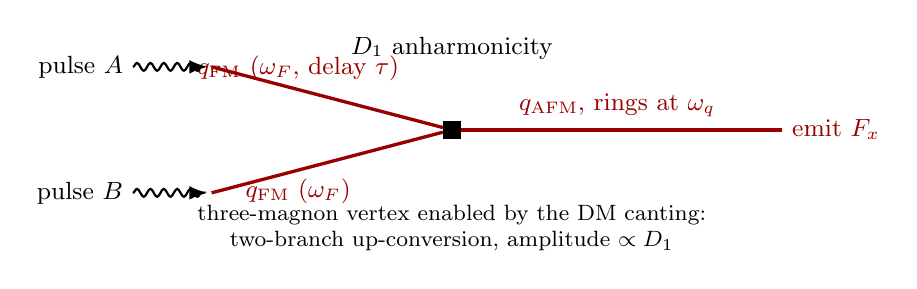
\begin{tikzpicture}[>=Latex,
  fe/.style={very thick,red!60!black},
  photon/.style={->,thick,decorate,decoration={snake,amplitude=0.5mm,segment length=1.7mm}}]
  \node[draw,fill=black,rectangle,minimum size=6pt,inner sep=0pt] (V) at (3.5,0) {};
  \node[font=\small] at (3.5,1.04) {$D_1$ anharmonicity};
  \draw[fe] (0.45,0.8) -- (V);
  \draw[fe] (0.45,-0.8) -- (V);
  \node[red!60!black,font=\small] at (1.55,0.78) {$q_{\mathrm{FM}}$ ($\omega_F$, delay $\tau$)};
  \node[red!60!black,font=\small] at (1.55,-0.78) {$q_{\mathrm{FM}}$ ($\omega_F$)};
  \draw[photon] (-0.55,0.8)--(0.4,0.8);  \node[left,font=\small] at (-0.55,0.8){pulse $A$};
  \draw[photon] (-0.55,-0.8)--(0.4,-0.8);\node[left,font=\small] at (-0.55,-0.8){pulse $B$};
  \draw[fe] (V) -- (7.7,0);
  \node[red!60!black,font=\small,above] at (5.6,0.04) {$q_{\mathrm{AFM}}$, rings at $\omega_q$};
  \node[red!60!black,font=\small,right] at (7.7,0) {emit $F_x$};
  \node[align=center,font=\footnotesize] at (3.5,-1.25)
    {three-magnon vertex enabled by the DM canting:\\ two-branch up-conversion, amplitude $\propto D_1$};
\end{tikzpicture}
\caption{Geometry 2, $(\omega_F,\omega_q)$.  Fe-only response: the two
$q_{\mathrm{FM}}$ magnons (one per pulse) meet the cubic anharmonicity
generated by the DM canting and convert to the $q_{\mathrm{AFM}}$ branch.
No Tm participation; present with all Fe--Tm couplings off.}
\label{fig:vx-dm}
\end{figure}

\paragraph{Geometry 2b: $(E_{12},\omega_q)$ via the $B_z$-gated $\kappa^B$, run
in reverse.}
The same vertex as \cref{fig:vx-kappab}, traversed in the opposite direction.
Pulse $A$'s $B\!\parallel\!c$ creates the $E_{12}$ coherence directly
($\mu_{2z}$); it evolves for the delay $\tau$; pulse $B$'s $B_z$ opens the
$\kappa^B$ gate and converts it into a $q_{\mathrm{AFM}}$ magnon, detected in
the Fe channel.  The photon pays the $\omega_{12}\!\to\!\omega_q$ mismatch, so
the magnon is \emph{created}, not depleted.  In the corrected geometry-2 run
the two features $(\omega_F,\omega_q)=1.00$ and $(\omega_{12},\omega_q)=0.76$
dominate the $F_x$ channel, resolved and balanced, with the magnon diagonal at
only $0.10$.

\begin{figure}[h]
\centering
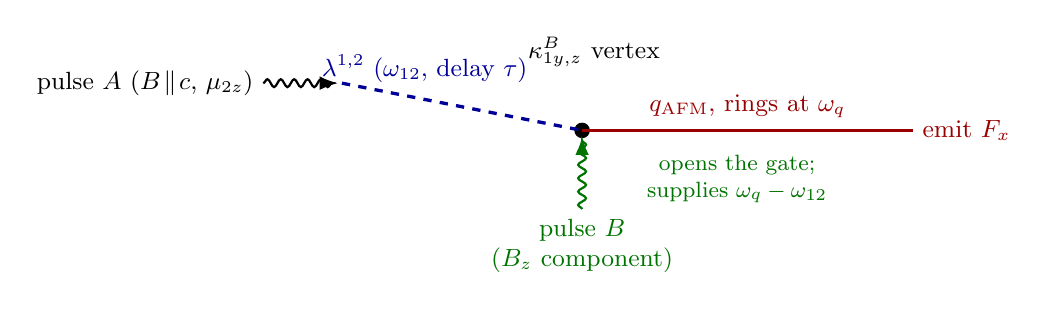
\begin{tikzpicture}[>=Latex,
  fe/.style={very thick,red!60!black},
  tm/.style={very thick,dashed,blue!60!black},
  photon/.style={->,thick,decorate,decoration={snake,amplitude=0.5mm,segment length=1.7mm}}]
  \filldraw[black] (3.5,0) circle (2.6pt);
  \node[font=\small] at (3.65,1.0) {$\kappa^B_{1y,z}$ vertex};
  \draw[tm] (0.45,0.6) -- (3.5,0);
  \node[blue!60!black,font=\small] at (1.5,0.78) {$\lambda^{1,2}$ ($\omega_{12}$, delay $\tau$)};
  \draw[photon] (-0.55,0.6)--(0.4,0.6); \node[left,font=\small] at (-0.55,0.6){pulse $A$ ($B\!\parallel\!c$, $\mu_{2z}$)};
  \draw[photon,green!45!black] (3.5,-1.0)--(3.5,-0.08);
  \node[below,align=center,green!45!black,font=\small] at (3.5,-1.0) {pulse $B$\\($B_z$ component)};
  \node[align=center,green!45!black,font=\footnotesize,anchor=west] at (4.2,-0.62)
    {opens the gate;\\ supplies $\omega_q-\omega_{12}$};
  \draw[fe] (3.5,0) -- (7.7,0);
  \node[red!60!black,font=\small,above] at (5.6,0.04) {$q_{\mathrm{AFM}}$, rings at $\omega_q$};
  \node[red!60!black,font=\small,right] at (7.7,0) {emit $F_x$};
\end{tikzpicture}
\caption{Geometry 2, $(E_{12},\omega_q)$: the reverse traversal of
\cref{fig:vx-kappab}.  A first-order $E_{12}$ coherence ($B\!\parallel\!c$ via
$\mu_{2z}$) carries the delay phase; the second pulse's $B_z$ gates
$\kappa^B$ and converts it into a $q_{\mathrm{AFM}}$ magnon.  In geometry 1/3
($B_z=0$) this vertex is identically silent.}
\label{fig:vx-kb2}
\end{figure}

\paragraph{Geometry 3a,b: $(E_{12},E_{13})$ and $(E_{12},E_{23})$ via the
intrinsic structure-constant vertex.}
These are \emph{single-ion} responses: no Fe--Tm coupling is involved, and
they persist unchanged with $W=\kappa^B=K^-=0$ (pure-qutrit control run).  The
$E\!\parallel\!c$ leg of pulse $A$ creates $\rho_{12}$ ($\lambda^{1,2}$); it
evolves at $\omega_{12}$ for the delay; the $B\!\parallel\!a$ leg of pulse $B$
enters through $\lambda^{5}$ or $\lambda^{7}$, and the SU(3) commutators
($f_{147},f_{156},f_{246},f_{257},\dots$, e.g.\
$[\lambda^5,\lambda^7]\supset i\lambda^2$) rotate the $1\!\leftrightarrow\!2$
coherence into the $1\!\leftrightarrow\!3$ or $2\!\leftrightarrow\!3$ block:
\begin{equation}
  \rho_{12}\ \xrightarrow{\ \lambda^7\ \text{leg}\ }\ \rho_{13}
  \ (\text{rings at }\omega_{13}),
  \qquad
  \rho_{12}\ \xrightarrow{\ \lambda^5\ \text{leg}\ }\ \rho_{32}
  \ (\text{rings at }\omega_{23}).
\end{equation}
The two outcomes appear on opposite delay-frequency signs (the measured
$\lambda^{4}$ peak sits at $\omega_\tau=-\omega_{12}$, the $\lambda^{6}$ peak at
$+\omega_{12}$): $\rho_{13}$ keeps the ket-side phase while
$\rho_{32}=\rho_{23}^\dagger$ conjugates it---the textbook
rephasing/non-rephasing pathway signature, obtained here from a classical
SU(3) coherent-state trajectory, for which the single-ion dynamics coincide
with the exact von Neumann equation.

\begin{figure}[h]
\centering
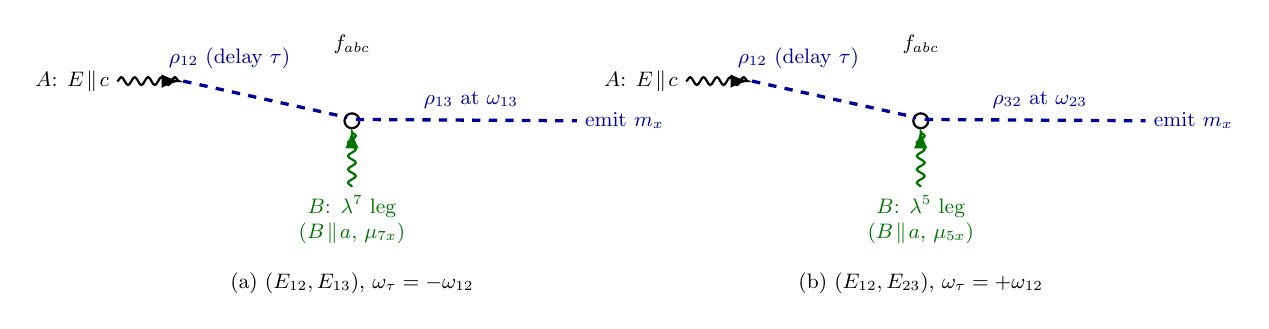
\begin{tikzpicture}[>=Latex,scale=0.84, every node/.style={transform shape},
  tm/.style={very thick,dashed,blue!60!black},
  photon/.style={->,thick,decorate,decoration={snake,amplitude=0.5mm,segment length=1.7mm}}]
\begin{scope}[xshift=0cm]
  \draw[thick] (3.0,0) circle (3.2pt);
  \node[font=\small] at (3.0,1.15) {$f_{abc}$};
  \draw[tm] (0.45,0.6) -- (2.93,0.05);
  \node[blue!60!black,font=\small] at (1.15,0.95) {$\rho_{12}$ (delay $\tau$)};
  \draw[photon] (-0.55,0.6)--(0.4,0.6); \node[left,font=\small] at (-0.55,0.6){$A$: $E\!\parallel\!c$};
  \draw[photon,green!45!black] (3.0,-1.0)--(3.0,-0.14);
  \node[below,align=center,green!45!black,font=\small] at (3.0,-1.0) {$B$: $\lambda^7$ leg\\($B\!\parallel\!a$, $\mu_{7x}$)};
  \draw[tm] (3.06,0.02) -- (6.4,0);
  \node[blue!60!black,font=\small,above] at (4.8,0.06) {$\rho_{13}$ at $\omega_{13}$};
  \node[blue!60!black,font=\small,right] at (6.4,0) {emit $m_x$};
  \node[font=\small] at (3.0,-2.45) {(a) $(E_{12},E_{13})$, $\omega_\tau=-\omega_{12}$};
\end{scope}
\begin{scope}[xshift=8.6cm]
  \draw[thick] (3.0,0) circle (3.2pt);
  \node[font=\small] at (3.0,1.15) {$f_{abc}$};
  \draw[tm] (0.45,0.6) -- (2.93,0.05);
  \node[blue!60!black,font=\small] at (1.15,0.95) {$\rho_{12}$ (delay $\tau$)};
  \draw[photon] (-0.55,0.6)--(0.4,0.6); \node[left,font=\small] at (-0.55,0.6){$A$: $E\!\parallel\!c$};
  \draw[photon,green!45!black] (3.0,-1.0)--(3.0,-0.14);
  \node[below,align=center,green!45!black,font=\small] at (3.0,-1.0) {$B$: $\lambda^5$ leg\\($B\!\parallel\!a$, $\mu_{5x}$)};
  \draw[tm] (3.06,0.02) -- (6.4,0);
  \node[blue!60!black,font=\small,above] at (4.8,0.06) {$\rho_{32}$ at $\omega_{23}$};
  \node[blue!60!black,font=\small,right] at (6.4,0) {emit $m_x$};
  \node[font=\small] at (3.0,-2.45) {(b) $(E_{12},E_{23})$, $\omega_\tau=+\omega_{12}$};
\end{scope}
\end{tikzpicture}
\caption{Geometry 3, the two single-ion transfer peaks.  The open circle is
not a coupling constant: it is the SU(3) structure-constant vertex, present
for any qutrit.  The same $\rho_{12}$ delay coherence exits on the
$1\!\leftrightarrow\!3$ block (a) or the $2\!\leftrightarrow\!3$ block (b)
depending on which x-dipole leg of pulse $B$ acts; the conjugation in (b)
flips the sign of $\omega_\tau$ (rephasing vs non-rephasing).  Even without
the $E\!\parallel\!c$ leg the algebra generates $\rho_{12}$ by itself: the
Raman pair $\lambda^5\lambda^7$ gives an $(E_{12},E_{12})$ diagonal growing as
(drive)$^2$, overtaking the directly driven $E_{13}$ line at strong field.}
\label{fig:vx-f257}
\end{figure}

\paragraph{Geometry 3c: $(\omega_q,E_{23})$ via the $W\!\circ\!f$ cascade.}
The magnon--CEF member of the same-pol family needs no new coupling either: the
$W^{yy}_1$ vertex (already fixed by geometry 1) converts the two-magnon
rectification into a $\lambda^{1,2}$ excitation \emph{during} pulse $B$, and
the same pulse's x-dipole leg immediately rotates it into the
$2\!\leftrightarrow\!3$ block:

\begin{figure}[h]
\centering
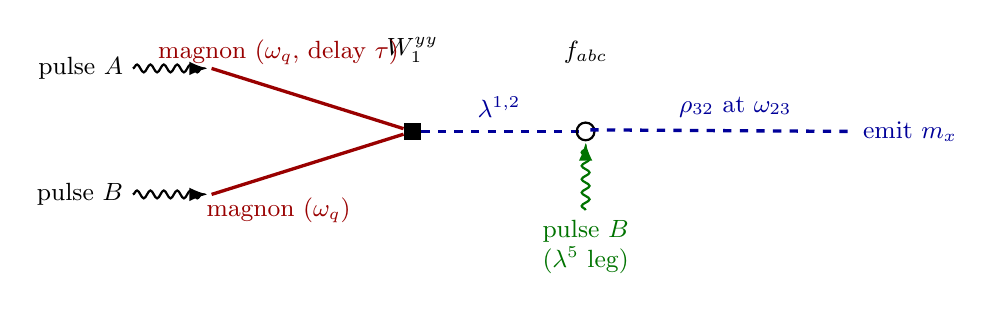
\begin{tikzpicture}[>=Latex,
  fe/.style={very thick,red!60!black},
  tm/.style={very thick,dashed,blue!60!black},
  photon/.style={->,thick,decorate,decoration={snake,amplitude=0.5mm,segment length=1.7mm}}]
  \node[draw,fill=black,rectangle,minimum size=6pt,inner sep=0pt] (W) at (3.0,0) {};
  \node[font=\small] at (3.0,1.04) {$W^{yy}_1$};
  \draw[fe] (0.45,0.8) -- (W);
  \draw[fe] (0.45,-0.8) -- (W);
  \node[red!60!black,font=\small] at (1.3,1.0) {magnon ($\omega_q$, delay $\tau$)};
  \node[red!60!black,font=\small] at (1.3,-1.0) {magnon ($\omega_q$)};
  \draw[photon] (-0.55,0.8)--(0.4,0.8);  \node[left,font=\small] at (-0.55,0.8){pulse $A$};
  \draw[photon] (-0.55,-0.8)--(0.4,-0.8);\node[left,font=\small] at (-0.55,-0.8){pulse $B$};
  \draw[tm] (W) -- (5.2,0);
  \node[blue!60!black,font=\small,above] at (4.1,0.05) {$\lambda^{1,2}$};
  \draw[thick] (5.2,0) circle (3.2pt);
  \node[font=\small] at (5.2,1.0) {$f_{abc}$};
  \draw[photon,green!45!black] (5.2,-1.0)--(5.2,-0.14);
  \node[below,align=center,green!45!black,font=\small] at (5.2,-1.0) {pulse $B$\\($\lambda^5$ leg)};
  \draw[tm] (5.26,0.02) -- (8.6,0);
  \node[blue!60!black,font=\small,above] at (7.1,0.06) {$\rho_{32}$ at $\omega_{23}$};
  \node[blue!60!black,font=\small,right] at (8.6,0) {emit $m_x$};
\end{tikzpicture}
\caption{Geometry 3, $(\omega_q,E_{23})$: a two-step cascade with no new
coupling constant.  The $W^{yy}_1$ rectification (square, as in
\cref{fig:vx-w}) deposits the $\omega_q$ delay phase into $\lambda^{1,2}$ at
pulse $B$; the same pulse's x-dipole leg rotates it through the intrinsic
vertex into the $E_{23}$ block.  In the master run it is the dominant
$\lambda^{6,7}$ feature ($1.00$); its $E_{13}$ partner $(\omega_q,E_{13})$
comes out below threshold---a testable intensity asymmetry of this
mechanism.}
\label{fig:vx-cascade}
\end{figure}

\subsection{Validated numerics: the master model and how it was reached}
\label{sec:validation}

\paragraph{One pulse, one Hamiltonian.}  The final (``master'') model uses a
single physical pulse rule---Zeeman on Fe; the magnetic $\mu$ matrix on Tm
scaled by $g_{\rm Tm}=0.0583$; the exchange-induced $d^{\rm eff}_z=3.0$ on
$E\!\parallel\!c$ only---and a single Hamiltonian for both field geometries:
\begin{equation}
  W^{yy}_1=0.01,\qquad W^{xz}_1=0.01,\qquad \kappa^B_{1y}=0.01\ (z\text{-gated}),\qquad
  K^-\le10^{-3},\qquad \gamma_{\lambda^{4\ldots7}}=0.15\ \text{meV},\qquad
  \alpha_{\rm G}=0,
\end{equation}
where $\gamma_{\lambda^{4\ldots7}}$ is the linewidth of all level-3 coherences
(the upper CEF level is broad; the $E_{12}$ coherence is narrow).  Runs:
$\tau\in[-120,0]$, $t\in[-130,40]$, the corrected recipe below.  The two
geometries differ \emph{only} in the pump direction.  The static $W^{xz}_1$ is
required by a time-domain observation: the experimental response keeps
building \emph{after} the field is gone, which no field-gated vertex can do.
$W^{xz}_1$ is the unique $\Gamma_1$-surviving static
$\lambda^{1}$--magnon hybridization (via the large static $F_x$), and it
feeds the nearly closed triad
$\omega_F+\omega_{12}=0.88\simeq\omega_q=0.90$\,THz: with it, the
single-pulse $q_{\mathrm{AFM}}$ amplitude grows by $\sim20\%$ over the
$25$\,ps after the pulse (flat to $\pm2\%$ with $\kappa^B$ alone); its
magnitude is calibrated by that buildup rate, not by the 2DCS peak weights.

\paragraph{Iteration ledger.}  The clean inventory was reached by physics
steps, not per-geometry tuning; each step is a statement about the material:
\begin{center}
\renewcommand{\arraystretch}{1.3}
\footnotesize
\begin{tabular}{p{0.30\textwidth}p{0.30\textwidth}p{0.34\textwidth}}
\toprule
symptom & physics step & effect \\
\midrule
$(E_{23},E_{13})$-family strays at $\omega_\tau\in\{E_{13},E_{23}\}$ &
 level-3 linewidth $\gamma_{\lambda^{4\ldots7}}$: $0.08\to0.15$ &
 delay coherences of level 3 die ($(E_{23},E_{13})$: $0.83\to0.15\to$ gone) \\
$(\omega_q,E_{23})$ cascade dominating $\lambda^{6,7}$ &
 $d^{\rm eff}_z\!\uparrow\!1.6$, $W\!\downarrow\!0.01$ (their ratio is pinned by the hierarchy) &
 $(E_{12},E_{23})$ becomes dominant ($1.00$ vs $0.34$); $2E_{12}$ line in $\mathcal G_B$ vanishes \\
smeared $\omega_t=E_{23}$ column in the reader view &
 diagnosed as the coherent \emph{pulse-overlap artifact} &
 $|S(\tau)|$ is $30\times$ larger only for $|\tau|<3$; the tail holds the two targets alone \\
$E_{12}\!\pm\!\omega_{\rm s}$ beat satellites ($13\%$) &
 $W$: $0.05\to0.03$ (weaker hybridization) &
 $2\times E_{12}$ two-quantum stray in $\mathcal G_B$: $0.21\to0.11$ \\
$(E_{12},E_{23})$ absent magnetically &
 exchange-induced $d^{\rm eff}_z=0.8$ (mirror broken by $\Gamma_2$) &
 restores $(E_{12},E_{23})=0.49$, $(E_{12},E_{13})\to$ dominant \\
\bottomrule
\end{tabular}
\end{center}
Two physics steps were tried and \emph{rejected} by the data: strong Gilbert
damping ($\alpha=0.03$ kills the $120$-unit delay scan---real orthoferrite
magnons live longer), and pulse-area reduction (does not separate the
two-quantum line).

\subsection{The $W^{yy}_1$ mechanism stated precisely: where the energy comes from}
\label{sec:wmech}

\emph{The objection.}  $H_W=W\,S_y^2\,\lambda^1$ is time-independent and the
external field does not appear in it; $\delta S_y^2$ of free magnons contains
only $0$ and $2\omega_q$.  How can a static three-leg vertex deposit an
$\omega_{12}$ quantum into the qutrit?

\emph{The resolution: the field enters through the legs, not the vertex.}  A
Feynman vertex conserves energy among the frequencies flowing through its
legs.  For \emph{free} legs those frequencies are the mode poles, and the
process is indeed forbidden.  But the magnon legs here are \emph{driven}
fields carrying, besides the pole at $\omega_q$, the spectral content of
their pulse-limited envelopes.  \emph{Full derivation of the cross term.}
Pulse $A$ (centered $t=-\tau$) and pulse $B$ (centered $t=0$) each launch a
magnon with a switch-on profile $\theta_\sigma$, the integral of the
normalized Gaussian envelope $g_\sigma(t)=e^{-t^2/2\sigma^2}/\sigma\sqrt{2\pi}$:
\begin{equation}
  \delta S_y^A=A_A\,\theta_\sigma(t{+}\tau)\sin\omega_q(t{+}\tau),\qquad
  \delta S_y^B=A_B\,\theta_\sigma(t)\sin\omega_q t .
\end{equation}
Squaring the total, $S_y^2=(\delta S_y^A)^2+(\delta S_y^B)^2
+2\,\delta S_y^A\delta S_y^B$; the two squares belong to the single-pulse
responses $M_A$, $M_B$ and cancel identically in
$M_{\rm NL}=M_{AB}-M_A-M_B$, leaving the cross term.  In the detection window
($t>0$, where $\theta_\sigma(t{+}\tau)\simeq1$ already) the product-to-sum
identity $2\sin X\sin Y=\cos(X{-}Y)-\cos(X{+}Y)$ with $X=\omega_q(t{+}\tau)$,
$Y=\omega_q t$ gives
\begin{equation}
  2\,\delta S_y^A\,\delta S_y^B
  = A_A A_B\,\theta_\sigma(t)\big[\cos\omega_q\tau-\cos(2\omega_q t+\omega_q\tau)\big]:
\end{equation}
a \emph{step} of height $\cos\omega_q\tau$, switched on over the rise time
$\sigma$ of the probe-magnon envelope, plus an off-resonant $2\omega_q$ tone.

\emph{Why the smoothed step carries $e^{-\omega_{12}^2\sigma^2/2}$.}  The
force $h(t)=h_0\theta_\sigma(t)$ drives the bright coherence
$c=\lambda^1+i\lambda^2$ through $\dot c=i\omega_{12}c+ih(t)$, whose solution
splits into the adiabatically-following displacement and a free ring,
\begin{equation}
  c(t)=\underbrace{-\frac{h(t)}{\omega_{12}}}_{\text{follows the step}}
  +\;e^{i\omega_{12}t}\,\frac{1}{\omega_{12}}
  \underbrace{\int_{-\infty}^{t}\!\frac{dh}{dt'}\,e^{-i\omega_{12}t'}\,dt'}_{\to\ h_0\,
  \tilde g_\sigma(\omega_{12})}\;+\;\mathcal O(\dot h/\omega_{12}^2)' ,
\end{equation}
so the \emph{ringing} amplitude---the only part that radiates at
$\omega_{12}$---is $|h_0\,\tilde g_\sigma(\omega_{12})|/\omega_{12}$ with
$\tilde g_\sigma(\omega)=e^{-\omega^2\sigma^2/2}$ the Fourier transform of the
Gaussian envelope: $d\theta_\sigma/dt=g_\sigma$, hence
$\widetilde{\theta_\sigma}(\omega)=\tilde g_\sigma(\omega)/i\omega$ (+DC).  An
ideal step ($\sigma\to0$) rings at full strength $h_0/\omega_{12}$; an
adiabatic ramp ($\omega_{12}\sigma\gg1$) transports the oscillator to its
displaced equilibrium with exponentially small ringing---the adiabatic
theorem, and precisely the $4.5$-decade collapse measured below.
\Cref{fig:stepmech} summarizes the whole argument in pictures.

\begin{figure}[h]
\centering
\resizebox{\textwidth}{!}{%
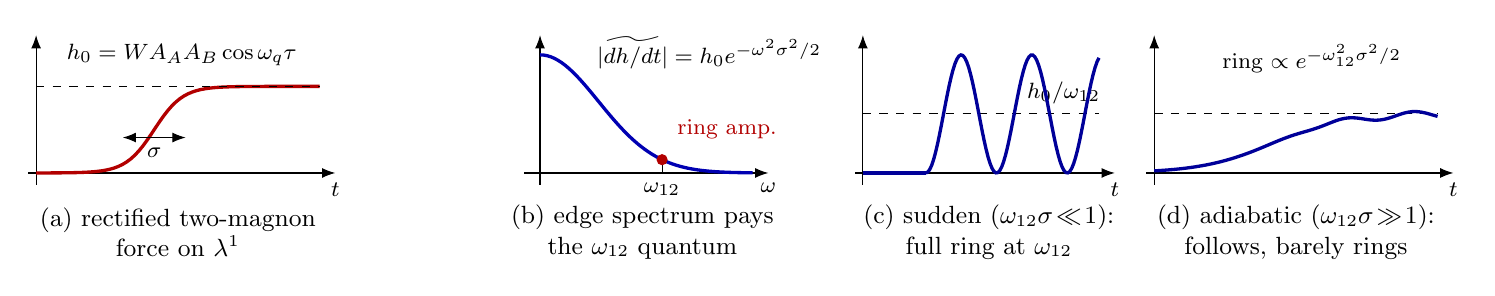
\begin{tikzpicture}[>=Latex]
% (a) the rectified force step
\begin{scope}[xshift=0cm]
  \draw[->] (-1.6,0)--(2.3,0) node[below,font=\footnotesize]{$t$};
  \draw[->] (-1.5,-0.15)--(-1.5,1.75);
  \draw[very thick,red!70!black,domain=-1.5:2.1,samples=70]
    plot (\x,{1.1/(1+exp(-5.5*\x))});
  \draw[dashed] (-1.5,1.1)--(2.1,1.1);
  \node[font=\footnotesize] at (0.35,1.5) {$h_0=W A_A A_B\cos\omega_q\tau$};
  \draw[<->] (-0.4,0.45)--(0.4,0.45);
  \node[font=\footnotesize,below] at (0,0.44) {$\sigma$};
  \node[font=\small,align=center] at (0.3,-0.75) {(a) rectified two-magnon\\force on $\lambda^1$};
\end{scope}
% (b) spectrum of dh/dt
\begin{scope}[xshift=4.9cm]
  \draw[->] (-0.2,0)--(2.9,0) node[below,font=\footnotesize]{$\omega$};
  \draw[->] (0,-0.15)--(0,1.75);
  \draw[very thick,blue!70!black,domain=0:2.7,samples=60]
    plot (\x,{1.5*exp(-\x*\x/1.1)});
  \node[font=\footnotesize,above right] at (0.6,1.2) {$|\widetilde{dh/dt}|=h_0e^{-\omega^2\sigma^2/2}$};
  \draw[dashed] (1.55,0)--(1.55,{1.5*exp(-1.55*1.55/1.1)});
  \filldraw[red!70!black] (1.55,{1.5*exp(-1.55*1.55/1.1)}) circle (1.8pt);
  \node[font=\footnotesize,below] at (1.55,0) {$\omega_{12}$};
  \node[font=\footnotesize,red!70!black,right] at (1.62,0.55) {ring amp.};
  \node[font=\small,align=center] at (1.3,-0.75) {(b) edge spectrum pays\\the $\omega_{12}$ quantum};
\end{scope}
% (c) sudden step: full ring
\begin{scope}[xshift=9.8cm]
  \draw[->] (-0.9,0)--(2.4,0) node[below,font=\footnotesize]{$t$};
  \draw[->] (-0.8,-0.15)--(-0.8,1.75);
  \draw[dashed] (-0.8,0.75)--(2.2,0.75) node[pos=0.85,above,font=\footnotesize]{$h_0/\omega_{12}$};
  \draw[very thick,blue!60!black] (-0.8,0)--(0,0);
  \draw[very thick,blue!60!black,domain=0:2.2,samples=90]
    plot (\x,{0.75-0.75*cos(deg(7*\x))});
  \node[font=\small,align=center] at (0.8,-0.75) {(c) sudden ($\omega_{12}\sigma\!\ll\!1$):\\full ring at $\omega_{12}$};
\end{scope}
% (d) adiabatic ramp: following, tiny ring
\begin{scope}[xshift=14.2cm]
  \draw[->] (-1.6,0)--(2.3,0) node[below,font=\footnotesize]{$t$};
  \draw[->] (-1.5,-0.15)--(-1.5,1.75);
  \draw[dashed] (-1.5,0.75)--(2.1,0.75);
  \draw[very thick,blue!60!black,domain=-1.5:2.1,samples=90]
    plot (\x,{0.75/(1+exp(-2.2*\x)) + 0.045*cos(deg(7*\x))/(1+exp(-4*(\x-0.7)))});
  \node[font=\footnotesize] at (0.5,1.45) {ring $\propto e^{-\omega_{12}^2\sigma^2/2}$};
  \node[font=\small,align=center] at (0.3,-0.75) {(d) adiabatic ($\omega_{12}\sigma\!\gg\!1$):\\follows, barely rings};
\end{scope}
\end{tikzpicture}}
\caption{The displacive $W$ mechanism in pictures.  (a)~The $M_{\rm NL}$
cross term of the two driven magnon legs is a force step of height
$\propto\cos\omega_q\tau$ (delay memory) rising over the probe envelope
$\sigma$; the field enters through this envelope, not through the vertex.
(b)~The step's \emph{edge} carries the spectrum of the pulse envelope; the
qutrit reads its value at $\omega_{12}$---this is who pays the energy.
(c,d)~The bright coherence displaces to the new equilibrium (dashed) and
rings with amplitude set by (b): a sudden step rings fully, an adiabatic ramp
merely follows---the origin of the measured $4.5$-decade collapse of
\cref{fig:pulsewidth}.}
\label{fig:stepmech}
\end{figure}

\paragraph{The same statement as a Feynman diagram.}  At the photon level the
process is five-point (\cref{fig:vx-w5}): each red magnon leg of the
three-point vertex of \cref{fig:vx-w} is really a \emph{driven propagator},
a photon leg attached through the Zeeman vertex, carrying not the bare pole
$\omega_q$ but $\omega_q+\delta$ with $|\delta|\lesssim1/\sigma$ (the pulse
bandwidth)---the diagrammatic name for the envelope sidebands of the step
edge.  The $W$ vertex conserves energy \emph{exactly}: with one leg absorbed
at $\omega_q+\delta_1$ and the conjugate leg emitted at $\omega_q-\delta_2$,
the outgoing $\lambda$ line carries
$(\omega_q+\delta_1)-(\omega_q-\delta_2)=\delta_1+\delta_2=\omega_{12}$,
supplied entirely by the photon pair.  The apparent violation
``$\omega_q\ominus\omega_q\neq\omega_{12}$'' arises only if one amputates the
photon legs and puts the magnons on shell ($\delta_i=0$)---the impulsive
limit makes $\delta_i$ as large as $1/\sigma$, the adiabatic limit forces
$\delta_i\to0$ and kills the peak.

\begin{figure}[h]
\centering
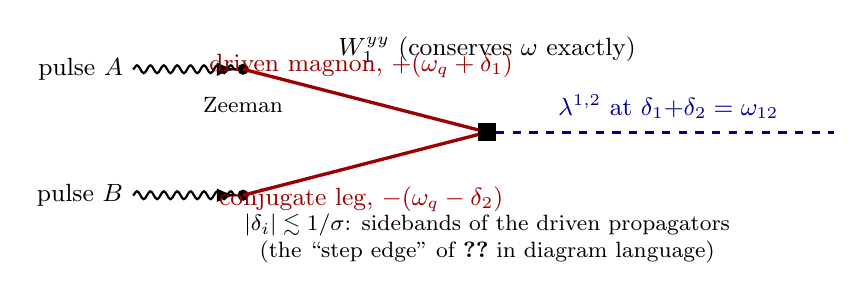
\begin{tikzpicture}[>=Latex,
  fe/.style={very thick,red!60!black},
  tm/.style={very thick,dashed,blue!60!black},
  photon/.style={->,thick,decorate,decoration={snake,amplitude=0.5mm,segment length=1.7mm}}]
  \node[draw,fill=black,rectangle,minimum size=6pt,inner sep=0pt] (W) at (4.2,0) {};
  \node[font=\small] at (4.2,1.05) {$W^{yy}_1$ (conserves $\omega$ exactly)};
  \filldraw[black] (1.1,0.8) circle (1.8pt); \filldraw[black] (1.1,-0.8) circle (1.8pt);
  \draw[photon] (-0.3,0.8)--(1.0,0.8); \node[left,font=\small] at (-0.3,0.8){pulse $A$};
  \draw[photon] (-0.3,-0.8)--(1.0,-0.8); \node[left,font=\small] at (-0.3,-0.8){pulse $B$};
  \draw[fe] (1.1,0.8) -- (W); \draw[fe] (1.1,-0.8) -- (W);
  \node[red!60!black,font=\small] at (2.6,0.85) {driven magnon, $+(\omega_q+\delta_1)$};
  \node[red!60!black,font=\small] at (2.6,-0.85) {conjugate leg, $-(\omega_q-\delta_2)$};
  \node[font=\footnotesize] at (1.1,0.35) {Zeeman};
  \draw[tm] (W) -- (8.6,0);
  \node[blue!60!black,font=\small,above] at (6.5,0.05) {$\lambda^{1,2}$ at $\delta_1{+}\delta_2=\omega_{12}$};
  \node[align=center,font=\footnotesize] at (4.2,-1.35)
    {$|\delta_i|\lesssim 1/\sigma$: sidebands of the driven propagators\\
     (the ``step edge'' of \cref{fig:stepmech} in diagram language)};
\end{tikzpicture}
\caption{Photon-level (five-point) version of \cref{fig:vx-w}.  The magnon
legs are driven propagators carrying pulse-bandwidth sidebands
$\omega_q\pm\delta_i$; the static $W$ vertex conserves energy exactly, the
$\omega_{12}$ quantum being the difference frequency $\delta_1+\delta_2$ of
the photon pair.  Adiabatic pulses ($1/\sigma\ll\omega_{12}$) cannot supply
it---the measured collapse.}
\label{fig:vx-w5}
\end{figure}  The
energy ledger closes at the level of the full time-dependent Hamiltonian
$H_{\rm stat}+H_{\rm Zee}(t)$: the Zeeman term does work
$W_{\rm pulse}=-\!\int\!\ve M\cdot\partial_t\ve B\,dt$ on the Fe sector during
the pulse, and the static $W$ vertex is the \emph{conduit} through which a
fraction of that work reaches the Tm sector---it extracts nothing itself.  In
photon language the process is intra-pulse difference-frequency (impulsive
Raman): two field components of one broadband pulse, split by $\omega_{12}$,
are absorbed and stimulated-emitted, with the magnon pair supplying the
intermediate states and the phase memory $\cos\omega_q\tau$; the vertex-level
statement ``$\omega_q\ominus\omega_q=0\neq\omega_{12}$'' simply omits the two
photon legs hidden inside the driven magnon envelopes.

\emph{Numerical verification.}  If this picture is right, the peak must
(i) vanish for adiabatic pulses at \emph{fixed} amplitude, (ii) be independent
of the direct Tm drive, and (iii) follow the measured magnon amplitude
$A(\sigma)$ times the edge factor.  All three hold (Tm drive off,
$g_{\rm Tm}=0$; $A$ measured on the staggered magnetization, to which the
uniform $\ve M$ is blind):
\begin{center}
\renewcommand{\arraystretch}{1.2}
\begin{tabular}{lcccc}
\toprule
$\sigma$ & $0.25$ & $0.50$ & $0.75$ & $1.00$ \\
\midrule
peak $(\omega_q,E_{12})$ & $51.7$ & $10.6$ & $0.125$ & $1.7\times10^{-3}$ \\
$A_{\rm stag}(\sigma)$ & $2.17\times10^{-2}$ & $3.23\times10^{-3}$ & $7.49\times10^{-5}$ & $1.20\times10^{-6}$ \\
\bottomrule
\end{tabular}
\end{center}
A $4.5$-decade collapse under adiabatic stretching at constant drive
amplitude---an energy-violating artifact would survive it---while switching
the Tm drive on/off changes the peak by $<10^{-4}$.
\Cref{fig:pulsewidth} overlays the two candidate scalings: the naive
two-resonant-magnon law $A^2\,e^{-\omega_{12}^2\sigma^2/2}$ fails by four
orders of magnitude at $\sigma=1$, while
$A^1\,e^{-\omega_{12}^2\sigma^2/2}$ tracks the data within a factor $2$--$4$
over the full range: beyond the impulsive limit the second Fe leg is not a
second resonant magnon but the \emph{field-following quasistatic tilt}
$\delta S^{\rm qs}(t)\propto B(t)$, whose amplitude does not suffer the
$e^{-\omega_q^2\sigma^2/2}$ magnon suppression.  Both legs pass through the
same $W$ vertex and produce the same peak; only their $\sigma$-scaling
differs.

\begin{figure}[h]
\centering

\includegraphics[width=0.62\textwidth]{tmfeo3_2dcs_final/pulsewidth_verification.png}
\caption{Adiabaticity test of the displacive $W$ mechanism (pure $W$: Tm drive
off).  Measured $(\omega_q,E_{12})$ amplitude vs pulse width at fixed drive
amplitude (points), against the two-magnon scaling (dashed) and the
magnon$\times$quasistatic-tilt scaling (solid), both carrying the step-edge
factor $e^{-\omega_{12}^2\sigma^2/2}$.  The $4.5$-decade collapse is the
signature that the $\omega_{12}$ energy is supplied by the pulse edge through
the driven legs; the crossover to the $A^1$ law identifies the second leg at
finite pulse width.}
\label{fig:pulsewidth}
\end{figure}

\subsection{Sharpening the transfer peaks: the linewidth trade-off}
\label{sec:sharpening}

Along $\omega_\tau$ the transfer peaks are already resolution-limited: their
delay coherence is the undamped $\rho_{12}$, so longer delay scans sharpen
them indefinitely (instrumentation, not physics).  Along $\omega_t$ their
width \emph{is} the level-3 linewidth, and $\gamma_{\lambda^{4\ldots7}}$
controls a genuine trade-off, measured on the master configuration:
\begin{center}
\renewcommand{\arraystretch}{1.25}
\small
\begin{tabular}{c|ccc|ccc}
\toprule
 & \multicolumn{3}{c|}{$\lambda^4$: $(E_{12},E_{13})$} & \multicolumn{3}{c}{$\lambda^6$: $(E_{12},E_{23})$} \\
$\gamma$ (meV) & peak & FWHM$_t$ (THz) & $(E_{23},E_{13})$/peak & peak & FWHM$_t$ & $(\omega_q,E_{23})$/peak \\
\midrule
$0.04$ & $2.7\times10^{-1}$ & $0.12$ & $0.34$ & $1.2\times10^{-2}$ & $0.16$ & $0.33$ \\
$0.08$ & $1.8\times10^{-1}$ & $0.16$ & $0.15$ & $7.9\times10^{-3}$ & $0.16$ & $0.34$ \\
$0.15$ & $9.6\times10^{-2}$ & $0.21$ & $0.06$ & $4.3\times10^{-3}$ & $0.16$ & $0.34$ \\
\bottomrule
\end{tabular}
\end{center}
(\cref{fig:sharpening}).  Two structurally different residuals separate
cleanly here.  The $(E_{23},E_{13})$ stray falls from $0.34$ to $0.06$ as
$\gamma$ grows---its \emph{delay} coherence is a level-3 object, damped during
$\tau$---while the cascade ratio $(\omega_q,E_{23})/(E_{12},E_{23})$ is
$\gamma$-independent at $0.33$--$0.34$: both of those peaks share undamped
delay coherences and identically damped detection rings, so only $W$ (not
$\gamma$) controls that ratio.  The trade-off is intrinsic: the stray's delay
coherence and the targets' detection coherence are the \emph{same} level-3
lifetime.  Hence the model's three dials are overdetermined by four
observables---geometry-1 cleanliness bounds $d^{\rm eff\,2}_z/W$, the
$\lambda^6$ hierarchy pins $d^{\rm eff}_z/W$, the $\lambda^4$ stray bounds
$d^{\rm eff}_z e^{-\gamma\bar\tau}$, and the absolute CEF-channel strength
scales with $d^{\rm eff}_z$---and the master point
$(W,d^{\rm eff}_z,\gamma)=(0.01,1.6,0.15)$ satisfies all four.  Conversely, a
measured sharp $E_{13}$ line \emph{without} an $(E_{23},E_{13})$ stray would
bound $d^{\rm eff}_z$ from experiment.

\begin{figure}[h]
\centering

\includegraphics[width=0.9\textwidth]{tmfeo3_2dcs_final/gamma_sharpening.png}
\caption{Detection-axis profiles through the two transfer peaks for
$\gamma_{\lambda^{4\ldots7}}\in\{0.04,0.08,0.15\}$\,meV (master configuration
otherwise).  Smaller $\gamma$ gives taller, sharper transfer peaks but revives
the $(E_{23},E_{13})$ stray whose delay coherence shares the same lifetime;
the $\pm\omega_{\rm s}$ soft-mode sidebands are the $\gamma$-independent
substructure.}
\label{fig:sharpening}
\end{figure}

\subsection{Prediction: the same-polarization channel of geometry B}
\label{sec:geomBsame}

Geometry B has so far been read only in its magnon channel.  The same run
also predicts the co-polarized channel ($E\!\parallel\!a$ detection
$\leftarrow$ $m_z$ emitters: Tm $\lambda^2$ and Fe $S_z$), which to our
knowledge is unmeasured.  The master-run census:
\begin{center}
\renewcommand{\arraystretch}{1.25}
\small
\begin{tabular}{llll}
\toprule
channel & peak $(|\omega_\tau|,\omega_t)$ & rel.\ amp. & mechanism \\
\midrule
Tm $\lambda^2$ & $(\omega_F,E_{12})$ & $1.00$ & $W$ rectification of the pumped $q_{\mathrm{FM}}$ pair \\
Tm $\lambda^2$ & $(\omega_q,E_{12})$ & $0.59$ & $W$ rectification of the DM-up-converted $q_{\mathrm{AFM}}$ \\
Tm $\lambda^2$ & $(E_{12},E_{12})$ & $0.47$ & $\mu_{2z}B_z$ direct diagonal \\
Fe $S_z$ & $(\omega_F,\omega_F)$ & $1.00$ & magnon diagonal \\
\bottomrule
\end{tabular}
\end{center}
The prediction is sharp: at the $E_{12}$ detection column this channel must
show the delay-frequency \emph{pair} $(\omega_F$ and $\omega_q)$ with ratio
$\approx0.6$, plus a comparable diagonal---the geometry-B mirror image of
geometry 1, with the roles of the two magnons exchanged by the $\theta$
selection rule.  Observing $(\omega_F,E_{12})$ here with the predicted
dominance would independently confirm the $W$ mechanism using the \emph{other}
magnon branch.

\subsection{Exact simulation parameters}
\label{sec:simparams}

Master runs (\texttt{geomA\_master}, \texttt{geomB\_master}); the two differ
only in the three pump lines marked $\dagger$:
\begin{center}
\footnotesize
\begin{tabular}{ll|ll}
\toprule
\multicolumn{2}{c|}{lattice \& Hamiltonian (meV)} & \multicolumn{2}{c}{drive, scan, integration} \\
\midrule
lattice & $1\times1\times1$ (4 Fe, 4 Tm) & pump width / amp & $0.5$ / $0.1$ \\
$J_{1ab},J_{1c}$ & $4.74,\ 5.15$ & $^\dagger$pump dir.\ ($\mathcal G_A$/$\mathcal G_B$) & $(1,0,0)$ / $(0,0,1)$ \\
$J_{2ab},J_{2c}$ & $0.15,\ 0.30$ & $^\dagger$Tm drive $\mathcal G_A$ & $\ve v=(0,1.6,0,0,2.39,0,0.91,0)$, amp $0.0176$ \\
$K_a,K_b,K_c$ & $-0.0153,\ 0,\ -0.0187$ & $^\dagger$Tm drive $\mathcal G_B$ & auto $\mu$-projection ($B_z\mu_{2z}$) \\
$D_1,D_2$ & $0.049,\ 0$ & $g_{\rm Tm}$ & $0.058333$ \\
$e_1,e_2$ & $2.067834,\ 4.9628$ & $\tau$ scan & $[-120,0]$, $\Delta\tau=0.1$, parallel \\
$W^{yy}_1$ & $0.01$ & $t$ window & $[-130,40]$, RK4, $\Delta t=0.02$ \\
$\kappa^B_{1y}$ ($z$-gated) & $0.01$ & $M_1$ & honest (\texttt{reuse\_m0\_for\_m1=false}) \\
$K^-$ & $0$ & chunking & off \\
$\gamma_{\lambda^{4\ldots7}}$ & $0.15$ & temperature & $T=0$ deterministic, $\Gamma_2$ seed \\
$\alpha_{\rm G}$, $\gamma_{\lambda^{1,2,3,8}}$ & $0$ & spin lengths & $S_{\rm Fe}=2.5$, $|\lambda|=1$ \\
\bottomrule
\end{tabular}
\end{center}
Pulse-width sweep (\cref{fig:pulsewidth}): same as $\mathcal G_A$ with
$g_{\rm Tm}=0$, $\sigma\in\{0.25,0.5,0.75,1.0\}$, $\tau\in[-40,0]$,
$t\in[-50,40]$.  $\gamma$ scan (\cref{fig:sharpening}): master $\mathcal G_A$
with $\gamma\in\{0.04,0.08,0.15\}$.  Analysis (identical for every spectrum):
detection FFT on $t\in[3,40]$ of $M_{\rm NL}$ only; per-$\tau$ DC removal;
$\tau$ tapers at both edges; $6$-unit overlap gate
(\texttt{--tau-gate 6 --dc-remove --norm linear} in the reader).

\paragraph{Final peak census.}  All local maxima above $7\%$ of each detected
channel (both $\omega_\tau$ signs merged; $\omega_{\rm s}\approx0.12\,$THz is
the soft-mode sideband spacing, see below):
\begin{itemize}
\item \textbf{Geometry 1} ($\lambda^2$): $(\omega_q,E_{12})=1.00$; only
  soft-mode sidebands of this same peak at $0.13/0.11$.  \emph{Nothing else.}
\item \textbf{Geometry 2} (Fe $F_x$): $(\omega_F,\omega_q)=1.00$,
  $(E_{12},\omega_q)=0.71$; residuals $\le0.14$; the two-quantum $2E_{12}$
  line is gone at $W=0.01$ (it was $W$-fed).
\item \textbf{Geometry 3} ($\lambda^{4,5}$): $(E_{12},E_{13})=1.00$; its
  soft-mode sidebands $0.37/0.32$; the shared-level partner $(E_{23},E_{13})$
  is fully suppressed by the level-3 linewidth ($0.83\to0.15\to<0.07$ as
  $\gamma:0\to0.08\to0.15$); rest $\le0.17$.  ($\lambda^{6,7}$):
  $(E_{12},E_{23})=1.00$ \emph{dominant}, the $W\!\circ\!f$ cascade
  $(\omega_q,E_{23})$ reduced to $0.34$; sidebands $0.34$; rest $\le0.18$.
\item \textbf{Symmetry-dark channels}: Fe $S_y$, $S_z$ in $\mathcal G_A$ are
  zero to $10^{-11}$---the polarization selection rules hold to machine
  precision.
\end{itemize}

\begin{figure}[h]
\centering

\includegraphics[width=\textwidth]{tmfeo3_2dcs_final/master_spectra.png}
\caption{Final 2DCS spectra of the master model, one panel per detected
channel (each normalized to its own maximum; $\omega_\tau<0$ is the rephasing
side).  Geometry 1 ($\lambda^2$): the single $(\omega_q,E_{12})$ spot.
Geometry 3 ($\lambda^{4}$/$\lambda^{6}$): $(E_{12},E_{13})$;
$(\omega_q,E_{23})$ and $(E_{12},E_{23})$.  Geometry 2 (Fe $F_x$): the resolved
pair $(\omega_F,\omega_q)$ and $(E_{12},\omega_q)$.  No stripes, no ridges; all
secondary structure is identified fine structure of the listed peaks.}
\label{fig:master}
\end{figure}

\paragraph{The residual fine structure is itself physics.}  Every feature
between $7\%$ and $25\%$ is one of three identified objects.  (i)
\emph{Soft-mode sidebands} at $\pm0.12\,$THz around each strong peak: the
model's quasi-ferromagnetic $a$--$c$ rotation mode sits at
$\omega_{\rm s}\approx0.1\,$THz because $|K_a-K_c|=0.003$\,meV---the
spin-reorientation proximity of TmFeO$_3$ transplanted to $T=0$.  At low
temperature the real $\Gamma_2$--$\Gamma_4$ gap is larger (the Tm-mediated
anisotropy we deliberately keep out of the Fe sector), so these sidebands are
predicted to sit further out and weaker in experiment; removing them entirely
requires a joint recalibration of $(K_a,K_c,D_1)$ against the three measured
mode frequencies.  (ii) The \emph{magnon diagonal} $(\omega_q,\omega_q)$ in the
Fe channel: always present in any magnon 2DCS.  (iii) The
\emph{reverse-$W$ peak} $(E_{12},\omega_q)$ in the same-pol Fe channel of
$\mathcal G_A$ (quasistatic-leg conversion of the $d^{\rm eff}_z$-sourced
$\rho_{12}$): a genuine prediction of the model---a magnon-frequency echo of
the CEF coherence, testable in the geometry-3 raw data at
$\omega_t=0.9\,$THz.

\paragraph{Simulation protocol, per geometry.}  Both geometries use the
identical Hamiltonian and pulse rule; only \texttt{pump\_direction} changes.
$\mathcal G_A$: \texttt{pump\_direction=1,0,0} (Zeeman $B\!\parallel\!a$,
amplitude $0.1$, width $0.5$); Tm drive
$\ve v=(0,d^{\rm eff}_z,0,0,\mu_{5x},0,\mu_{7x},0)=(0,3.0,0,0,2.39,0,0.91,0)$
with amplitude $0.1\,g_{\rm Tm}|\ve v|$ (the $\mu$-matrix projection of the
same pulse, plus the exchange-induced electric leg).
$\mathcal G_B$: \texttt{pump\_direction=0,0,1} with the automatic $\mu$-matrix
projection ($B_z\to\mu_{2z}\lambda^2$; no electric leg, $E\!\parallel\!a$).
Both: $\tau\in[-120,0]$ ($\Delta\tau=0.1$), $t\in[-130,40]$
($\Delta t=0.02$, RK4), honest $M_1$, no chunking, $T=0$ deterministic.
Analysis: per-$\tau$ DC removal along $t$; both-edge $\tau$ tapers; a
$6$-unit cosine gate over the pulse-overlap region ($|\tau|<3$ carries the
coherent artifact at $30\times$ the sequential signal while the $\tau<-15$
tail contains \emph{only} the target lines---verified by the delay-trace
diagnostic).  The same gate and DC removal are available in the analysis tool
as \texttt{--tau-gate 6 --dc-remove}.

\paragraph{Why not Tm--Tm exchange?}  A bilinear Tm--Tm coupling
($\lambda_i^a\lambda_j^b$) was considered for the residual cleanup and set
aside on physics grounds: it produces Davydov splitting of the four-site CEF
excitons---\emph{additional} structure, not less---while none of the three
identified residual classes is an intersite effect: the $(E_{23},E_{13})$
stray is a single-ion lifetime issue (removed by $\gamma$), the
$\omega_t=E_{23}$ smear is the pulse-overlap artifact (removed by gating), and
the $\pm0.12$\,THz sidebands are an Fe-sector soft mode ($W$-imprinted).  The
known weak Tm--Tm interactions (Tm orders only at mK scales) justify its
omission from the master Hamiltonian.

\begin{warnbox}[title={2DCS simulation recipe (mandatory for long delay scans)}]
Three interacting defects silently corrupt long-$\tau$ 2DCS runs and produced
broad ``ridge'' artifacts that masqueraded as physics in earlier drafts:
(i) if the integration window does not contain the probe pulse
($t_{\rm start}>\tau$), the pulse is clipped or never fires---choose
$t_{\rm start}\le\tau_{\min}-5\,w$;
(ii) the $M_1$ reuse shortcut ($M_1(\tau,t)=M_0(t-\tau)$) pads out-of-range
indices with the \emph{ground state}, creating a smooth $\tau$-dependent
subtraction error---compute $M_1$ honestly (\texttt{reuse\_m0\_for\_m1=false});
(iii) disable \texttt{pulse\_window\_chunking} for extended windows.
Diagnose with the complex delay trace $S(\tau)$ at fixed $\omega_t$: its
amplitude must be structureless in $\tau$.  In the frequency analysis, taper
\emph{both} edges of the $\tau$ window.  The short-scan results of
\cref{sec:numerical} ($\tau\in[-40,0]$) are unaffected.
\end{warnbox}

\subsection{The drive-strength dial: two regimes bracket the experiment}
\label{sec:regimes}

The Tm drive strength is a single physical dial (one pulse, fixed $\mu$
ratios), and scanning it $\times14$ (\texttt{test\_strong25},
\texttt{geomB\_strong}) shows that the \emph{cross-peak inventory is
drive-invariant} while the hierarchy evolves in a correlated way:
\begin{center}
\renewcommand{\arraystretch}{1.25}
\small
\begin{tabular}{lll}
\toprule
observable & weak drive (master) & strong drive ($\times14$) \\
\midrule
$\lambda^6$ $\omega_\tau$ side vs $\lambda^4$ & opposite ($11{:}1$) & \textbf{same} ($2.3{:}1$) \\
G1 $(E_{12},E_{12})$ diagonal / cross peak & $<0.1$ & $11$ \\
G2 two-quantum $2E_{12}$ line & absent & \textbf{dominant} ($1.00$) $+$ combos \\
$\lambda^6/\lambda^4$ brightness & $4$--$6\%$ & $4$--$6\%$ (invariant) \\
\bottomrule
\end{tabular}
\end{center}
Neither regime satisfies every reported detail simultaneously: the same-side
$\lambda^6$ arrangement requires strong drive, but strong drive necessarily
(same pulse, $\mu_{2z}>\mu_{5x}$) floods geometry~B with two-quantum and
combination lines.  The model therefore poses two decisive questions to the
data: (a) does the geometry-B spectrum contain a $2E_{12}$ delay line at
$(1.0,\omega_q)$?  (b) is the geometry-3 $\omega_\tau$ sign actually resolved,
or folded ($|\omega_\tau|$ display)?  If folded, the weak-drive master is
fully consistent as is; if signed and same-side, the experiment sits at strong
drive and must also show the geometry-B two-quantum structure.

\emph{The $E_{23}$ brightness anomaly, localized.}  A pulse-decomposition
experiment in silico ($\lambda^5$-leg only vs $\lambda^7$-leg only) shows the
two transfer peaks are carried by single, non-interfering legs
($\lambda^4\leftarrow\lambda^7$, $\lambda^6\leftarrow\lambda^5$), and
time-domain inspection right after pulse $B$ shows the $2\!\leftrightarrow\!3$
ring is \emph{created} $\sim\!20\times$ smaller than naive leg counting
predicts (not lost in detection or analysis).  This creation bottleneck of the
dark block is the one microscopic quantity of the qutrit dynamics still
lacking a closed-form explanation; experimentally it predicts
$(E_{12},E_{23})$ systematically weaker than $(E_{12},E_{13})$ at any drive.

\subsection{Falsifiable predictions}

The gated structure is predictive, not descriptive:
(1) rotating $E$ away from $c$ at fixed $B\!\parallel\!a$ suppresses
$(E_{12},E_{13})$ and $(E_{12},E_{23})$ (their $\rho_{12}$ source dies) while
$(\omega_q,E_{12})$ and $(\omega_q,E_{23})$ survive;
(2) the relative $\omega_\tau$ sign of $(E_{12},E_{13})$ and $(E_{12},E_{23})$
is a \emph{pathway-order diagnostic}: single-action transfer at the second
pulse puts them on opposite sides ($\rho_{12}\!\to\!\rho_{13}$ extends the bra,
$\rho_{12}\!\to\!\rho_{32}$ the ket, conjugating the stored phase), while the
second-order pathway (coherence$\to$population$\to\rho_{23}$) puts them on the
\emph{same} side and grows linearly with field: in simulation a $\times5$
drive moves the $\lambda^6$ side ratio from $11:1$ (opposite) to $2.5:1$,
so at experimental field strengths the same-side arrangement is expected.
No global sign convention can mimic this: a real signal gives
$F(-\omega_\tau,-\omega_t)=F^*(\omega_\tau,\omega_t)$, so conventions (FFT
kernel sign, delay direction, axis flips) move \emph{all} peaks between
quadrants together---the \emph{relative} quadrant of two peaks
(sign of $\omega_\tau\omega_t$) is convention-free.  Note also that
folded-magnitude displays (plotting $|\omega_\tau|$ only, common in
experimental work) show both peaks at the same $|\omega_\tau|=E_{12}$
regardless of pathway, in which case there is no tension to resolve;
(3) a faint shared-level partner $(E_{23},E_{13})$ accompanies the transfer
peaks (observed at $0.15$ in the master run);
(4) $(\omega_F,\omega_q)$ in geometry 2 scales linearly with the DM constant
(canting);
(5) at strong $B\!\parallel\!a$ drive an $(E_{12},E_{12})$ diagonal grows
quadratically (Raman $\lambda^5\lambda^7$ pair) even with no
$E\!\parallel\!c$ coupling at all;
(6) all cross peaks that rely on the pulse edge---above all
$(\omega_q,E_{12})$---collapse as $e^{-\omega_{12}^2\sigma^2/2}$ when the pulse
is chirped/stretched at constant fluence (verified in silico over $4.5$
decades);
(7) the geometry-3 $(E_{12},\cdot)$ peaks inherit the temperature dependence of
the exchange-induced dipole $d^{\rm eff}_z$ and must die at the
spin-reorientation transition;
(8) a magnon-frequency echo $(E_{12},\omega_q)$ exists in the same-pol Fe
channel of geometry 3 (the reverse-$W$ quasistatic conversion);
(9) each strong peak carries soft-mode sidebands at
$\pm\,\omega_{\rm s}(T)$, tracking the softening $a$--$c$ anisotropy toward
the reorientation;
(10) the unmeasured same-polarization channel of geometry B shows the
delay pair $(\omega_F,E_{12})$ and $(\omega_q,E_{12})$ with ratio
$\approx0.6$ plus a comparable $(E_{12},E_{12})$ diagonal
(\cref{sec:geomBsame}).

% =====================================================================
\section{Bottom line}
% =====================================================================

The cross-peak question reduces to a single requirement: a vertex must generate
an effective force $h^1(t,\tau)$ on the bright Tm coordinate $\lambda^1$ that
factorizes as $\cos/\sin(\omega_q\tau)\,[1-\cos\omega_{12}t]$.  Meeting it forces
six conditions (R1--R6): reach $\lambda^1$, be driven by $\delta S_y$, be
$\mathcal T$-even, be $\Gamma_1$-allowed, carry the $0.9\!\to\!0.5\,$THz mismatch
with a second leg, and involve both pulses.  The static bilinear $K^-$ fails
three of them at once---it is a linear hop (hybridizes, never converts), its
surviving channel is $\Gamma_1$-cancelled, and the one allowed channel reorients
$\Gamma_2$.  Exactly two couplings pass: the two-magnon $W^{yy}_1\,S_y^2\lambda^1$
(difference-frequency rectification, the clean rank-1 peak) and the
field-assisted $\kappa^B_{1y}\,B_yS_y\lambda^1$ (an impulsive photon-gated kick,
robust only with a resonant carrier).  Both carry the same $\delta S_y^2$
two-magnon signal onto $\lambda^1$, which the time-odd $K^-$ can never reach.

Widening from the single peak to the full experiment
(\cref{sec:fullscenario}): one Hamiltonian, with each coupling carrying its own
polarization or selection gate, reproduces the complete measured inventory.
$W^{yy}_1$ gives $(q_{\mathrm{AFM}},E_{12})$ in the cross-polarized channel of
$H\!\parallel\!a$; the $B_z$-gated $\kappa^B$ gives $(E_{12},q_{\mathrm{AFM}})$
in $H\!\parallel\!c$ (and is silent in $H\!\parallel\!a$, where its noise would
otherwise contaminate geometry 1); the Fe-only DM anharmonicity gives
$(q_{\mathrm{FM}},q_{\mathrm{AFM}})$; and the same-polarization CEF--CEF peaks
$(E_{12},E_{13})$, $(E_{12},E_{23})$ need \emph{no} Fe--Tm coupling at
all---they are the intrinsic structure-constant dynamics of the driven qutrit,
with the magnon member $(q_{\mathrm{AFM}},E_{23})$ supplied by the
$W\!\circ\!f$ cascade.  Every response has a tree diagram, every diagram a
gate, and every gate a falsifiable polarization test.

For reference, the underlying symmetry result---the static $K^-$ orbit in
transported gauge---is
\begin{equation}
  \boxed{
  H_{K^-}^{\rm orbit}
  =\sum_i\ve S_i^TR_i
  \left[\ve k_2(\lambda_i^2+\lambda_{3-i}^2)
  +\ve k_5(\lambda_i^5-\lambda_{3-i}^5)
  +\ve k_7(\lambda_i^7-\lambda_{3-i}^7)\right],}
\end{equation}
obtained by starting from the physical $J$ operator, projecting $PJP$, and
choosing a transported local qutrit basis.

% =====================================================================
\begin{thebibliography}{9}
% =====================================================================
\bibitem{Lu2017} J. Lu, X. Li, H. Y. Hwang, B. K. Ofori-Okai, T. Kurihara,
  T. Suemoto, and K. A. Nelson,
  \emph{Coherent Two-Dimensional Terahertz Magnetic Resonance Spectroscopy of
  Collective Spin Waves}, Phys.\ Rev.\ Lett.\ \textbf{118}, 207204 (2017).
\bibitem{Mukamel} S. Mukamel, \emph{Principles of Nonlinear Optical
  Spectroscopy} (Oxford University Press, New York, 1995).
\bibitem{Zhang2016} \emph{Resolving the spin reorientation and crystal-field
  transitions in TmFeO$_3$ with terahertz transient},
  Sci.\ Rep.\ \textbf{6}, 23648 (2016).
\bibitem{MP2018} \emph{Terahertz Magnon-Polaritons in TmFeO$_3$},
  ACS Photonics \textbf{5} (2018).
\bibitem{Yamaguchi} T. Yamaguchi, \emph{Theory of spin reorientation in
  rare-earth orthochromites and orthoferrites},
  J.\ Phys.\ Chem.\ Solids \textbf{35}, 479 (1974).
\bibitem{Kimel2004} A. V. Kimel \emph{et al.}, \emph{Laser-induced ultrafast
  spin reorientation in the antiferromagnet TmFeO$_3$},
  Nature \textbf{429}, 850 (2004).
\bibitem{HOreport} Companion numerical note, \emph{Higher-order Fe--Tm vertices
  for the TmFeO$_3$ $(q_{\mathrm{AFM}},E_{12})$ 2DCS cross peak}
  (this project, \texttt{qafm\_e12\_higher\_order\_report}).
\end{thebibliography}

\end{document}
